\documentclass[a4paper,11pt,fleqn,twoside,openright]{memoir} % Brug openright hvis chapters skal starte p� h�jresider; openany, oneside
%\usepackage{fancyhdr}%mega nemt sidehoved/fod%virker ikke med memoir �benbart
%%%% PACKAGES %%%%

%\usepackage[T1]{fontenc}
%\usepackage{pgfplots}%Ting til grafer (sat ind december 2012)
%\pgfplotsset{
%  compat=newest,
%  xlabel near ticks,
%  ylabel near ticks
%} Ting til grafer (sat ind december 2012)

\usepackage[english]{babel}							% Dansk sporg, f.eks. tabel, figur og kapitel
%\usepackage{pst-plot,pst-node}
%\usepackage[pdf]{pstricks} % G�r det muligt at tegne vektor grafik.
%\usepackage{auto-pst-pdf,pstricks-add}
% �� Overs�ttelse og tegns�tning �� %
%\usepackage[ansinew]{inputenc}					% G�r det muligt at bruge �, � og � i sine .tex-filer

%\usepackage[T1]{fontenc}								% Hj�lper med orddeling ved �, � og �. S�tter fontene til at v�re ps-fonte, i stedet for bmp					

% �� FONTS �� % LaTeX er fanme ringe til skrifttyper!
%\usepackage{txfonts}									% konflikter med et eller andet.. giver i hvert fald fejl
\usepackage{mathptmx}								% times (den vi normalt bruger - bare ingen fed mat skrift)
%\usepackage{fourier}									% s�dan lidt middle ground mellem times og pazo (har heller ikke mathbf)
%\usepackage{mathpazo}								% Har fed tekst i matematik (minus mathbf), grim almindelig skrift
%\usepackage{mtpro2}									% f�lger ikke med som standard, men hvis nogen kan installere det skal de da v�re velkomne

\usepackage{latexsym}										% LaTeX symboler
\usepackage{xcolor,ragged2e,fix-cm}			% Justering af elementer
\usepackage{pdfpages}										% G�r det muligt at inkludere pdf-dokumenter med kommandoen \includepdf[pages={x-y}]{fil.pdf}	
\pretolerance=2500 											% G�r det muligt at justre afstanden med ord (h�jt tal, mindre orddeling og mere space mellem ord)
\usepackage{ulem}                       % Gennemstregning af ord med koden \sout{}
\usepackage{fixltx2e}										% Retter forskellige bugs i LaTeX-kernen
\usepackage[shortlabels]{enumitem}			% Muligg�r enkelt konfiguration af lister
\usepackage{alltt}											% Bruges af highlighting (matlab kode)
%\usepackage{Lastpage}

%Matlab kode hightlighting
 \definecolor{string}{rgb}{0.7,0.0,0.0}
    \definecolor{comment}{rgb}{0.13,0.54,0.13}
    \definecolor{keyword}{rgb}{0.0,0.0,1.0}
											
%Include cpp coding in text
\usepackage{listings}
\usepackage{color}

\definecolor{dkgreen}{rgb}{0,0.6,0}
\definecolor{gray}{rgb}{0.5,0.5,0.5}
\definecolor{mauve}{rgb}{0.58,0,0.82}

\lstset{frame=tb,
  language=C++,  
  aboveskip=3mm,
  belowskip=3mm,
  showstringspaces=false,
  columns=flexible,
  basicstyle={\small\ttfamily},
  numbers=none,
  numberstyle=\tiny\color{gray},
  keywordstyle=\color{blue},
  commentstyle=\color{dkgreen},
  stringstyle=\color{mauve},
  breaklines=true,
  breakatwhitespace=true,
  tabsize=3
}											
																			
% �� Figurer og tabeller � floats  �� %
\usepackage{flafter}										% S�rger for at dine floats ikke optr�der i teksten f�r de er sat ind.
\usepackage{multirow}                		% Fletning af r�kker
\usepackage{hhline}                   	% Dobbelte horisontale linier
\usepackage{multicol}         	        % Fletning af kolonner
\usepackage{colortbl} 									% Mulig�re farver i tabeller
\usepackage{rotating}										% Muligg�r rotation af tekst i tabeller med \begin{sideways}...\end{sideways}
\usepackage{wrapfig}										% Inds�ttelse af figurer omsv�bt af tekst. \begin{wrapfigure}{Placering}{St�rrelse}
\usepackage{graphicx} 									% Pakke til jpeg/png billeder
%\pdfoptionpdfminorversion=6%							% Muligg�r inkludering af pdf dokumenter, af version 1.6 og h�jere
\usepackage{tabularx} %Muligg�r at man kan str�kke en tabel-kolonne til �nsket l�ngde
\newsubfloat{figure}
\usepackage{epstopdf}

% �� Matematiske formler og maskinkode ��
\usepackage{amsmath, amssymb} 	% Bedre matematik og ekstra fonte 
\usepackage{textcomp}                 	% Adgang til tekstsymboler
\usepackage{mathtools}									% Udvidelse af amsmath-pakken. 
\usepackage{eso-pic}										% Tilf�j billedekommandoer p� hver side
\usepackage{lipsum}											% Dummy text \lipsum[..]



% �� Referencer, bibtex og url'er �� %
\usepackage{url}												% Til at s�tte urler op med. Virker sammen med hyperref
\usepackage[english]{varioref}						% Giver flere bedre mulighed for at lave krydshenvisninger
%\usepackage{natbib}											% Litteraturliste med forfatter-�r og nummerede referencer
%\usepackage{cite} 												% G�r det muligt at nummere kilder
\usepackage{xr}													% Referencer til eksternt dokument med \externaldocument{<NAVN>}
\usepackage{nomencl}										% Pakke til at danne nomenklaturliste
\makenomenclature												% Nomenklaturliste


% �� Floats �� %
\let\newfloat\relax 										% Memoir har allerede defineret denne, men det g�r float pakken ogs�
\usepackage{float}

\usepackage[footnote,draft,english,silent,nomargin]{fixme}		% Inds�t rettelser og lignende med \fixme{...} Med final i stedet for draft, udl�ses en error 																															for hver fixme, der ikke er slettet, n�r rapporten bygges.

%%%% CUSTOM SETTINGS %%%%

% �� Marginer �� %
\setlrmarginsandblock{3.5cm}{2.5cm}{*}	% \setlrmarginsandblock{Indbinding}{Kant}{Ratio}
\setulmarginsandblock{2.5cm}{3.0cm}{*}	% \setulmarginsandblock{Top}{Bund}{Ratio}
\checkandfixthelayout 									% Laver forskellige beregninger og s�tter de almindelige l�ngder op til brug ikke memoir pakker

%	�� Afsnitsformatering �� %
\setlength{\parindent}{0mm}           	% St�rrelse af indryk
\setlength{\parskip}{4mm}          			% Afstand mellem afsnit ved brug af double Enter
\linespread{1,1}												% Linie afstand

% �� Litteraturlisten �� %
%\bibpunct[,]{[}{]}{;}{a}{,}{,} 					% Definerer de 6 parametre ved Harvard henvisning (bl.a. parantestype og seperatortegn)
%\bibliographystyle{bibtex/harvard}			% Udseende af litteraturlisten. Ligner dk-apali - mvh Klein

% �� Indholdsfortegnelse �� %
\setsecnumdepth{subsection}		 					% Dybden af nummerede overkrifter (part/chapter/section/subsection)
\maxsecnumdepth{subsection}							% �ndring af dokumentklassens gr�nse for nummereringsdybde
\settocdepth{subsection} 								% Dybden af indholdsfortegnelsen

% �� Lister �� %
\setlist{
  topsep=-1ex,														% Vertikal afstand mellem tekst og listen
  itemsep=-1ex,													% Vertikal afstand mellem items
  partopsep=-0ex,
  parsep=1ex
} 

% �� Visuelle referencer �� %
\usepackage[colorlinks]{hyperref}			 	% Giver mulighed for at ens referencer bliver til klikbare hyperlinks. .. [colorlinks]{..}
\hypersetup{pdfborder = 0}							% Fjerner ramme omkring links i fx indholsfotegnelsen og ved kildehenvisninger ��
\hypersetup{														%	Ops�tning af farvede hyperlinks
    colorlinks = false,
    linkcolor = black,
    anchorcolor = black,
    citecolor = black
}

\definecolor{gray}{gray}{0.80}					% Definerer farven gr�

% �� Ops�tning af figur- og tabeltekst �� %
 	\captionnamefont{
 		\small\bfseries\itshape}						% Ops�tning af tekstdelen ("Figur" eller "Tabel")
  \captiontitlefont{\small}							% Ops�tning af nummerering
  \captiondelim{. }											% Seperator mellem nummerering og figurtekst
  \hangcaption													%	Venstrejusterer flere-liniers figurtekst under hinanden
  \captionwidth{\linewidth}							% Bredden af figurteksten
	\setlength{\belowcaptionskip}{-15pt}		% Afstand under figurteksten
		
% �� Navngivning �� %
\addto\captionsenglish{
	\renewcommand\appendixname{Appendix}
	\renewcommand\contentsname{Table of Contents}	
	\renewcommand\appendixpagename{Appendix}
	\renewcommand\cftchaptername{\chaptername~}				% Skriver "Kapitel" foran kapitlerne i indholdsfortegnelsen
	\renewcommand\cftappendixname{\appendixname~}			% Skriver "Bilag" foran bilagene i indholdsfortegnelsen
	\renewcommand\appendixtocname{Appendix}
}

% �� Kapiteludssende �� %


\definecolor{numbercolor}{gray}{0.7}			% Definerer en farve til brug til kapiteludseende
\newif\ifchapternonum

\makechapterstyle{jenor}{									% Definerer kapiteludseende -->
  \renewcommand\printchaptername{}
  \renewcommand\printchapternum{}
  \renewcommand\printchapternonum{\chapternonumtrue}
  \renewcommand\chaptitlefont{\fontfamily{pbk}\fontseries{db}\fontshape{n}\fontsize{25}{35}\selectfont\raggedleft}
  \renewcommand\chapnumfont{\fontfamily{pbk}\fontseries{m}\fontshape{n}\fontsize{1in}{0in}\selectfont\color{numbercolor}}
  \renewcommand\printchaptertitle[1]{%
    \noindent
    \ifchapternonum
    \begin{tabularx}{\textwidth}{X}
    {\let\\\newline\chaptitlefont ##1\par} 
    \end{tabularx}
    \par\vskip-2.5mm\hrule
    \else
    \begin{tabularx}{\textwidth}{Xl}
    {\parbox[b]{\linewidth}{\chaptitlefont ##1}} & \raisebox{-15pt}{\chapnumfont \thechapter}
    \end{tabularx}
    \par\vskip2mm\hrule
    \fi
  }
}																						% <--

%BLUEBOX KAPITEL
\newsavebox{\ChpNumBox}
\definecolor{ChapBlue}{rgb}{1,0,0} % !!
\makeatletter
\newcommand*{\thickhrulefill}{%
\leavevmode\leaders\hrule height 1\p@ \hfill \kern \z@}
\newcommand*\BuildChpNum[2]{%
\begin{tabular}[t]{@{}c@{}}
\makebox[0pt][c]{#1\strut} \\[.5ex]
\colorbox{ChapBlue}{%
\rule[-10em]{0pt}{0pt}%
\rule{1ex}{0pt}\color{black}#2\strut
\rule{1ex}{0pt}}%
\end{tabular}}
\makechapterstyle{BlueBox}{%
\renewcommand{\chapnamefont}{\large\scshape}
\renewcommand{\chapnumfont}{\Huge\bfseries} 		
\renewcommand{\chaptitlefont}{\raggedright\Huge\scshape} % \bfseries
\setlength{\beforechapskip}{10pt}	%DEFAULT:20pt
\setlength{\midchapskip}{20pt}	%DEFAULT:26pt
\setlength{\afterchapskip}{15pt}	%DEFAULT:40pt !!
\renewcommand{\printchaptername}{}
\renewcommand{\chapternamenum}{}
\renewcommand{\printchapternum}{%
\sbox{\ChpNumBox}{%
\BuildChpNum{\chapnamefont\@chapapp}%
{\chapnumfont\thechapter}}}
\renewcommand{\printchapternonum}{%
\sbox{\ChpNumBox}{%
\BuildChpNum{\chapnamefont\vphantom{\@chapapp}}%
{\chapnumfont\hphantom{\thechapter}}}}
\renewcommand{\afterchapternum}{}
\renewcommand{\printchaptertitle}[1]{%
\usebox{\ChpNumBox}\hfill
\parbox[t]{\hsize-\wd\ChpNumBox-1em}{%
\vspace{\midchapskip}%
\thickhrulefill\par
\chaptitlefont ##1\par}}%
}


% Valg af kapiteludseende - dette kan udskiftes efter �nske
%\chapterstyle{madsen}	%P1-style		
\chapterstyle{BlueBox}									

% �� Sidehoved �� %

\makepagestyle{custom}		% Definerer sidehoved og sidefod - kan modificeres efter �nske -->
\makepsmarks{custom}{																						
\def\chaptermark##1{\markboth{\itshape\thechapter. ##1}{}}		% Henter kapitlet den p�g�ldende side h�rer under med kommandoen \leftmark. \itshape g�r teksten kursiv
\def\sectionmark##1{\markright{\thesection. ##1}{}}					% Henter afsnittet den p�g�ldende side h�rer under med kommandoen \rightmark
}																														% Sidetallet skrives med kommandoen \thepage	
\makeevenhead{custom}{Computational Physics}{}{\leftmark}							% Definerer lige siders sidehoved efter modellen \makeevenhead{Navn}{Venstre}{Center}{H�jre}
\makeoddhead{custom}{\rightmark}{}{University of Oslo}			% Definerer ulige siders sidehoved efter modellen \makeoddhead{Navn}{Venstre}{Center}{H�jre}
\makeevenfoot{custom}{\thepage}{}{}													% Definerer lige siders sidefod efter modellen \makeevenfoot{Navn}{Venstre}{Center}{H�jre}
\makeoddfoot{custom}{}{}{\thepage}														% Definerer ulige siders sidefod efter modellen \makeoddfoot{Navn}{Venstre}{Center}{H�jre}		
\makeheadrule{custom}{\textwidth}{0.5pt}											% Tilf�jer en streg under sidehovedets indhold
\makefootrule{custom}{\textwidth}{0.5pt}{1mm}								% Tilf�jer en streg under sidefodens indhold

\copypagestyle{nychapter}{custom}														% F�lgende linier s�rger for, at sidefoden bibeholdes p� kapitlets f�rste side
\makeoddhead{nychapter}{}{}{}
\makeevenhead{nychapter}{}{}{}
\makeheadrule{nychapter}{\textwidth}{0pt}
\aliaspagestyle{chapter}{nychapter}													% <--

\pagestyle{custom} %normalt plain% Valg af sidehoved og sidefod
\usepackage[left=2.4cm, right=2.4cm, top=3cm, bottom=3cm]{geometry}	%Overrider tidliger marginer - men det er lidt mere simpelt.

%%%% CUSTOM COMMANDS %%%%
%referencer
\newcommand{\figref}[1]{Fig.~\ref{#1}}
\newcommand{\tabref}[1]{Tab.~\ref{#1}}	
\newcommand{\matref}[1]{Eq.~\eqref{#1}}
\newcommand{\chapref}[1]{Chap.~\ref{#1}}
\newcommand{\secref}[1]{Sec.~\ref{#1}}
\newcommand{\subsecref}[1]{Subsec.~\ref{#1}}
\newcommand{\appref}[1]{App.~\ref{#1}}
\newcommand{\citer}[1]{\citep[Se][]{#1}}
\newcommand{\citerk}[2][]{\citep[Se][kap.~#1]{#2}}
\newcommand{\citers}[2][]{\citep[Se][s.~#1]{#2}}


% �� Billede hack �� %
\newcommand{\figur}[4]{
		\begin{figure}[H] \centering
			\includegraphics[width=#1\textwidth]{billeder/#2}
			\caption{#3}\label{#4}
		\end{figure} 
		}
		
% �� Specielle tegn �� %
\newcommand{\grader}{\ensuremath{^{\circ}\text{C}}}
\newcommand{\gr}{\ensuremath{^{\circ}}}
\newcommand{\g}{\cdot}


% �� Promille-hack (\promille) �� %
\newcommand{\promille}{%
  \relax\ifmmode\promillezeichen
        \else\leavevmode\(\mathsurround=0pt\promillezeichen\)\fi}
\newcommand{\promillezeichen}{%
  \kern-.05em%
  \raise.5ex\hbox{\the\scriptfont0 0}%
  \kern-.15em/\kern-.15em%
  \lower.25ex\hbox{\the\scriptfont0 00}}

\newcommand{\HRule}{\rule{\linewidth}{0.5mm}}

% �� CUSTOM MATEMATIK/FYSIK-TING ��
\renewcommand{\v}[1]{\ensuremath{\mbox{\textbf{#1}}}} % for vectors
\newcommand{\gv}[1]{\ensuremath{\mbox{\boldmath$ \vec{#1}  $}}} 
% for vectors of Greek letters
\newcommand{\uv}[1]{\ensuremath{\mbox{\boldmath$ \hat{#1}  $}}}  % for unit vector
\newcommand{\abs}[1]{\left| #1 \right|} % for absolute value
\newcommand{\avg}[1]{\left< #1 \right>} % for average
\let\underdot=\d % rename builtin command \d{} to \underdot{}
\renewcommand{\d}[2]{\frac{d #1}{d #2}} % for derivatives
\newcommand{\dd}[2]{\frac{d^2 #1}{d #2^2}} % for double derivatives
\newcommand{\pd}[2]{\frac{\partial #1}{\partial #2}} 
% for partial derivatives
\newcommand{\pdd}[2]{\frac{\partial^2 #1}{\partial #2^2}} 
% for double partial derivatives
\newcommand{\pdc}[3]{\left( \frac{\partial #1}{\partial #2}
 \right)_{#3}} % for thermodynamic partial derivatives
\newcommand{\ket}[1]{\left| #1 \right>} % for Dirac bras
\newcommand{\bra}[1]{\left< #1 \right|} % for Dirac kets
\newcommand{\braket}[2]{\left< #1 \vphantom{#2} \right|
 \left. #2 \vphantom{#1} \right>} % for Dirac brackets
\newcommand{\matrixel}[3]{\left< #1 \vphantom{#2#3} \right|
 #2 \left| #3 \vphantom{#1#2} \right>} % for Dirac matrix elements
\newcommand{\grad}[1]{\gv{\nabla} #1} % for gradient
\let\divsymb=\div % rename builtin command \div to \divsymb
\renewcommand{\div}[1]{\gv{\nabla} \cdot #1} % for divergence
\newcommand{\curl}[1]{\gv{\nabla} \times #1} % for curl
\let\baraccent=\= % rename builtin command \= to \baraccent
\renewcommand{\=}[1]{\stackrel{#1}{=}} % for putting numbers above =
\renewcommand\Re{\operatorname{Re}}
\renewcommand\Im{\operatorname{Im}}
\newcommand{\comp}[1]{\widetilde{#1}}
\newcommand{\unit}[1]{\ensuremath{\, \mathrm{#1}}}

\newcommand{\eqvref}[1]{(\ref{#1}) p� side \pageref{#1}}

\newcommand{\forsog}[1]{\underline{#1}}

\newcommand{\superscript}[1]{\ensuremath{^{\textrm{#1}}}}
\newcommand{\subscript}[1]{\ensuremath{_{\textrm{#1}}}}


%%%% ORDDELING %%%%

\hyphenation{egen-skab-er egen-skab hvad hvem hvor Halv-le-der-ud-snit-tet}

% Makro til fxnotes
\newcommand{\AVP}[1]{\fxnote{\textbf{AVP}: #1}}
\newcommand{\BM}[1]{\fxnote{\textbf{BM}: #1}}
\usepackage[font=small,labelfont=bf]{caption}  %package for figcap mm.
\raggedbottom
\begin{document}

\frontmatter	% Romertal på de første sider
\thispagestyle{empty}

\begin{center}


% Upper part of the page

\textsc{\LARGE University of Oslo}\\[0.5cm]

\textsc{\Large Computational Physics}\\[2cm]
 

% Title
\HRule \\[0.4cm]
 \LARGE \textbf{Project 5}  \\[0.2cm]
\HRule \\[2.5cm]

\vspace{2cm}

\includegraphics[width=0.8\textwidth]{Figures/UiO_Seal_A_ENG.png}\\  %Forsidebillede

\vfill 
 
% Forfattere og vejleder
\begin{tabularx}{\textwidth}{l X r}
\hline
& & \large \emph{Authors:}\\
& & \large Birgitte Madsen, 66\\
& & \large Magnus Isaksen, 14 \\
& & \large Soumya Chalakkal, 51 \\
\hline

\end{tabularx}




\vfill

% Bottom of the page
{\large Autumn 2015}

\end{center}
\cleardoublepage


\cleardoublepage		
% Dette er LaTeX-versionen af titelbladet for tek-nat-basis-rapporter 2004 efterår
% Filen kræver:
% Universitetets logo:  aau-logo.png (for LaTeX) eller aau-logo.ps (for LaTeX)
% Synopsis: En fil ved navn synopsis.tex

% Udarbejdet af: Hans HŸttel (hans@cs.auc.dk) 21. maj 2003
% Rettet af Morten Christophersen (mortench@tnb.aau.dk) 30. nov 2004(ændret til nyt design 2004 efterår)

%\documentclass[11pt]{article}
%\ifx\pdfoutput\undefined 
%\usepackage[dvips]{graphicx}
%\else
%\usepackage[pdftex]{graphicx} 
%\usepackage{type1cm} \fi
%    \usepackage[ansinew]{inputenc}
%    \usepackage{a4}

%\begin{document} 
\phantomsection
\pdfbookmark[0]{Titelblad}{titelblad}
\thispagestyle{empty}
%\begin{titlepage}
\begin{nopagebreak}
{\samepage 
\begin{tabular}{r}
\parbox{\textwidth}{  \raisebox{1mm}{
\includegraphics[height=1.5cm]{Figures/UiO_Seal_A_ENG.png}}
\hfill \parbox{5.5cm}{\begin{tabular}{r} %4.90
{\small \textbf{Department of Physics}}\\
{\small  \textbf{University of Oslo}} \\
{\small  Sem S\ae lands vei 24} \\
{\small  0371 Oslo, Norway} \\
{\small +47 22 85 64 28} \\
%{\small Fax 99 40 92 35} \\
{\small http://www.mn.uio.no/fysikk/english/}
\end{tabular}}}

\end{tabular}

\vspace{2.5cm}
\begin{tabular}{cc}
\parbox{20cm}{
\begin{description}
\item { \textbf{Course:}}

	Computational Physics\\
	\hspace{4cm}
	\vspace{0.7cm}
\item { \textbf{Project number:}}

	5 \\
	\hspace{4cm}
	\vspace{0.7cm}

\item {\textbf{Link to GitHub folder:} }

	\url{https://?????}  \\ 
	\hspace{4cm}
	\vspace{0.7cm}

\item { \textbf{Hand-in deadline:}}

   Friday, December 11, 2015\\
  \hspace{4cm}
  \vspace{0.7cm}
  
\item { \textbf{Project Members:}}

Birgitte Madsen, 66 \\
Magnus Isaksen, 14 \\
Soumya Chalakkal, 51 \\
  \hspace{2cm}
  \vspace{0.7cm}

\end{description}

\vspace{0.25cm}
\begin{description}
\item { \textbf{Copies:} 1}
\item { \textbf{Page count:} \pageref{LastPage}  } 
\item { \textbf{Appendices:} 0} 
\item { \textbf{Completed:} ????, 2015 } 
\end{description}
\vfill } &
%\parbox{7cm}{
%  \vspace{.15cm}
%  \hfill 
%  \begin{tabular}{l}
%  {\textbf{Synopsis:}}\bigskip \\
%  \fbox{
%    \parbox{6.5cm}{\bigskip
%     {\vfill{\small \input{Chapters/Formalia/synopsis.tex}
%     \bigskip}}
%     }}
%   \end{tabular}}
\end{tabular}}
\\ \\ \\ 

\noindent{\footnotesize{\textit{The content of the report is freely available, but publication (with source) may only be made with the agreement of the authors.}}}
\end{nopagebreak}
%\end{titlepage}
%\end{document}

\cleardoublepage
\chapter*{Abstract}

In this project an open cluster is simulated using two different algorithms, the fourth order Runge-Kutta and the Velocity Verlet. During the project the fourth order Runge-Kutta is chosen as the main algorithm, as it gives more stable results for a many body system. The evolution of the cluster is studied looking at the energies, the distribution of particles and positions as time progresses. Studying the energies it was found that the system lost energy as particles were ejected from the cluster. When the system reached an approximately equilibrium state after a period of $3\tau_{crunch}$, it was consistent with the virial theorem.

\cleardoublepage	
%\chapter*{Preface}
This project is written by 6th semester physics group 4.207a at the Department of Physics and
Nanotechnology at Aalborg University, Denmark, in the Spring semester, 2014, as a 10 ECTS-point bachelor project.

\subsection*{Reading Guide}
Succeeding chapters support each other, and it is therefore recommended to read the report chronologically.
When referring to equations or the like in the text, \textit{equation} will be shortened Eq., \textit{table} will be shortened Tab., and so forth.
In \appref{app:ListOfSymbols} a list of frequently used symbols and constants are given.
The external references used in this work appear in numbered order in brackets in the text and are listed in the bibliography at the end of the report in order of succession.

\subsection*{Signatures}
The group member's signatures below express that the entire group is accountable for all aspects of the project and all chapters of the report. 

\vspace{4cm}

\begin{table}[H]
	\centering
		\begin{tabular}{c c}
			\underline{\phantom{JAERJAERJAERJAERJAERJAERJAER}}	 	&	\underline{\phantom{JAERJAERJAERJAERJAERJAERJAER}} 
			\\
			Andreas V. Pedersen								& 	Birgitte Madsen	
			\\									
		\end{tabular}
\end{table}
%\cleardoublepage			
\tableofcontents*

\mainmatter % Side nummereringen starter ved 1 herfra

	\chapter{Introduction}

	\chapter{Method}
\label{chap:method} 
The methods introduced in this chapter, are used to study the evolution of bodies, also referred to as particles, in the solar system or in the galaxy. 
Firstly, the fourth order Runge-Kutta method and the Velocity-Verlet method are introduced for a 2-body problem in 3 dimensions, however, since the aim of this project is to investigate the time evolution of a star cluster consisting of $N$ particles, the code is extended to $N$ bodies by incorporating suitable changes. 

To generate the $N$ bodies, a function for generating the position coordinates of the N bodies as uniformly distributed particles within a sphere is introduced as discussed in sec \secref{Method:GeneratingPosMassVel}, along with a function for generating masses that are randomly distributed by a Gaussian distribution around ten solar masses with a standard deviation of one solar mass.

In the Github folder \url{https://github.com/birgimad/Project5_BM_MI_SC}, the source codes for the algorithms described in this chapter can be found. 


	\section{Transformation between units}
\label{sec:Conversion}
When considering at a planetary system or a larger system like a galaxy it is inconvenient to use the SI units for length and time.
Instead, to investigate the evolution of astronomical systems, it is an advantage to use days, years (yr) or even longer time periods as the unit of time, and astronomical units (AU) or light-years (ly) as the unit of distance.
The change in unit system, evidently changes the considered constant, the gravitational constant $G$, which in SI units is given as
\begin{align*}
	G = 6.67\cdot 10^{-11} \frac{\textrm{Nm}^2}{\textrm{kg}^2}
\end{align*}
For a planetary system like the Earth-Sun system it is better to consider distances in AU instead of meters, and use days as a measure of time, as the planet doesn't move far on its orbit in a second.
Furthermore it's an advantage to express the masses in the system in units of solar mass. 
Hence the constants have to be transformed into these unit systems. 

The gravitational constant G is transformed using
\begin{align*}
	1 \textrm{ AU} = 1.495\cdot10^{11} \textrm{ m}
	\qquad \text{and} \qquad
	1 \textrm{ M}_{\odot} = 1.989 \cdot 10^{30} \textrm{ kg}
\end{align*}
giving the gravitational constant for the planetary system
\begin{align*}
	G = 2.96\cdot 10^{-4} \frac{\textrm{AU}^3}{\textrm{days}^2 \textrm{M}_{\odot}}
\end{align*}
which is convenient when considering a planetary system.
 
For a star cluster the distances are greater and the time scales are larger than for the planetary system.
Therefore it's more convenient to use years as the unit of time and light-years (ly) as the unit of distance. 
\begin{align*}
	1 \textrm{ yr} = 3.1536\cdot10^7\textrm{s}
	\qquad \text{and} \qquad
	c = 2.008\cdot 10^8 \frac{\textrm{m}}{\textrm{s}}
\end{align*}
in which $c$ is the speed of light.
This yields that 1 ly is
\begin{align*}
	1 \textrm{ ly} = 9.45 \cdot 10^{15} \textrm{ m}
\end{align*}

Giving the gravitational constant for stellar distances 
\begin{align*}
	G = 1.536\cdot 10^{-13} \frac{\textrm{ly}^3}{\textrm{yr}^2 {\textrm{M}}_{\odot}}
\end{align*}



Finding the gravitational constant in units of $\tau:{chrunch}$. 
\begin{align*}
G = 986.96 \frac{\textrm{ly}^3}{\tau_{crunch}^2 \textrm{m}_{mean}}
\end{align*}


	\section{Newtonian two-body problem in three dimension}
\label{Newton2body3D}
The problem of solving the time-evolution of a two-body system in three dimensions can reasonably be considered in two different coordinate systems: one coordinate system with one of the bodies in rest compared to the frame of reference in which the other body is moving, and one coordinate system with both of the bodies moving relative to the frame of reference. 
Both of these reference systems are depicted in \figref{fig:2bodyproblem_coordinatesystems}. 
\begin{figure}[H]
\centering
	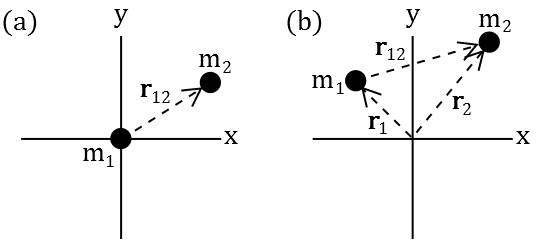
\includegraphics[width=0.6\linewidth]{Figures/2bodyproblem_coordinatesystems.png}
\caption{
Two-dimensional illustration of the three-dimensional problem of determining determining the relative distance and relative velocity between two bodies. 
In (a) body 1 with mass $m_1$ is considered stationary in position- and velocity-space, whilst body 2 with mass $m_2$ moves relative to body 1.
In (b) both body 1 and 2 moves relative to the frame of reference in position and time, yielding that the position vector between body 1 and 2 is given as $\v{r}_{12} = \v{r}_2 - \v{r}_1$.
}
\label{fig:2bodyproblem_coordinatesystems}
\end{figure}
In the codes presented in this section, solving the problem in coordinate system (a) will first be considered for simplicity. Thereafter, the codes will be extended to include the movement of body 1 relative to the coordinate system, since this will be useful when extending the codes to an N body system.  

In the problem, $\v{r}(t)$ is the three-dimensional space vector consisting of the coordinated $(x(t),y(t),z(t))$, whilst $\v{v}(t)$ is the three-dimensional velocity vector with coordinates $(v_x(t),v_y(t),v_z(t))$, both of which are dependent on time. 

In general, the considered differential equation is
\begin{align}
	\frac{dy}{dt} = f(t,y)
	\label{eq:diffEq1}
\end{align}
Which yields that
\begin{align}
	y(t) = \int f(t,y) dt
\end{align}
\fxnote{do we need to write $y_{i+1}$ eq from p. 250 in lecture notes??}
For the two bodies in a three dimensional Newtonian gravitational field this corresponds to six coupled differential equations given by the vector equations
\begin{align}
	\frac{d\v{r}}{dt} = \v{v}
	\qquad \text{and} \qquad
	\frac{d\v{v}}{dt} = - \frac{G M_1 M_2}{r^3} \v{r}
	\label{eq:diffEq2}
\end{align}
\fxnote{maybe we should divide by mass as on p. 248??}
in which $M_1$ and $M_2$ \fxnote{fix the this with $M_1$ and $M_2$} are the masses of the two bodies, respectively, whilst $r$ is the distance between the bodies.
The equations in \eqref{eq:diffEq2} are computed by the script given below in which $drdt$ corresponds to the derivative of the coordinates of the position, and $dvdt$ corresponds to the derivative of the velocity coordinates. 
\begin{lstlisting}
void Derivative(double r[3], double v[3], double (&drdt)[3], double (&dvdt)[3], double G, double mass){
    drdt[0] = v[0];
    drdt[1] = v[1];
    drdt[2] = v[2];

    double distance_squared = r[0]*r[0] + r[1]*r[1] + r[2]*r[2];
    double newtonian_force = -G*mass/pow(distance_squared,1.5);
    dvdt[0] = newtonian_force*r[0];
    dvdt[1] = newtonian_force*r[1];
    dvdt[2] = newtonian_force*r[2];
}
\end{lstlisting}

	\subsection{Velocity-Verlet method}
\label{sec:methodVV}
The basic idea of the Velocity-Verlet algorithm is to write the Taylor expansion of the position in Newton’s equation, one forward step and one backward step in time with step length $\delta t$ as
\begin{align}
	\v{r}(t_i \pm \delta t) = \v{r}(t_i) \pm \v{v} (t_i) \delta t
	+ \v{a} (t_i) \frac{\delta t ^2}{2}  \pm \frac{\delta t ^3}{6} \frac{d^3 \v{r}(t_i)}{dt^3} + \mathcal{O}(\delta t ^4 )
	\label{eq:TaylorExpVVmethod}
\end{align}
in which $\v{v}(t_i) = d\v{r}(t_i)/dt$ is the velocity, and $\v{a}(t_i) = d^2 \v{r}(t_i)/dt^2$ is the acceleration at time $t_i$.
Adding the two expressions in \matref{eq:TaylorExpVVmethod} gives
\begin{align}
	\v{r} (t_i +\delta t) = 2\v{r} (t_i) - \v{r} (t_i -\delta t)  + \v{a} (t_i ) \delta t^2 + \mathcal{O} (\delta t ^4 )
	\label{eq:TaylorExpVVmethod2}
\end{align}
which has a truncation error that goes as $\mathcal{O} (\delta t ^4 )$.
Now, using $\v{r}(t_i-\delta t) = \v{r}(t_i) - \v{v}(t_i) \delta t + \v{a} \delta t^2 /2 + \mathcal{O} (\delta t^3)$, yield that the position at time $t_i+\delta t$ can be determined as 
\begin{align}
	\v{r}(t_i+\delta t) = \v{r}(t_i) + \v{v} (t_i) \delta t + \frac{1}{2} \v{a} (t_i) \delta t^2 
	\label{eq:VVmethodNextPosition}
\end{align}
Since the velocity is not included in \matref{eq:TaylorExpVVmethod2}, it is computed through the Velocity-Verlet scheme where position, velocity and acceleration at time $t_i+\delta t$ is computed from the Taylor expansion as
\begin{align}
	\v{v} (t + \delta t) = \v{v} (t) + \frac{1}{2} ( \v{a} (t) + \v{a} (t + \delta t) ) \delta t
	\label{eq:VVmethodNextVelocity}
\end{align}
The velocity at time $t_i+\delta t$ is in the algorithm computed by first calculating 
\begin{align}
	\v{v}_{part1} (t + \delta t) = \v{v} (t) + \frac{1}{2}  \v{a} (t)  \delta t
	\label{eq:VVmethodNextVelocityPart1}
\end{align}
and then use the \textit{Derivative} function to determine $\v{a} (t + \delta t)$, which is then used to compute the remaining term of \matref{eq:VVmethodNextVelocity} as 
\begin{align}
	\v{v}_{part2} (t + \delta t) = \frac{1}{2} \v{a} (t + \delta t) \delta t
	\label{eq:VVmethodNextVelocityPart2}
\end{align}

The velocity-Verlet method uses the algortihm \textit{Derivative} described in \secref{Newton2body3D}, to generate the six differential equations, in the following while-loop that runs until reaching the final time in time steps of length $\delta t = (t_{initial} - t_{final})/(\# time steps)$.
\begin{lstlisting}
    while(time<=t_final){
    Derivative(r,v,drdt,dvdt,G,mass);
    for(int i=0; i<6 ; i++){
    r[i] = r[i]+dt*drdt[i] + 0.5 * dt * dt * dvdt[i];
    v_partly[i] = drdt[i] + 0.5 * dt * dvdt[i];
    dvdt[i] = v_partly[i];
    }
    Derivative(r,v,drdt,dvdt,G,mass);
    for(int i=0; i<n ; i++){
    v[i] = v_partly[i] + 0.5 * dt * dvdt[i];
    }
    time += dt;
    }
\end{lstlisting}	
	\subsection{Fourth Order Runge-Kutta Method}
\label{sec:methodRK4}
- Remember to write about accuracy of algorithm!!

The Runge-Kutta method is based on Taylor expansions, with the next function value after a times step $\delta t = t_i - t_{i+1}$ being computed from four more or less improved slopes of the function in the points $t_i$, $t_i + \delta t /2$ and $t_{i+1}$.
  
The first step of the RK4 method is to compute the slope $k_1$ of the function in $t_i$ by
\begin{align*}
	k_1 = \delta t f(t_i , y_i)
\end{align*}
Then the slope $k_1$ at the midpoint is computed from $k_1$ as
\begin{align*}
	k_2 = \delta t f(t_i + \delta t /2, y_i + k_1 /2 )
\end{align*}
The slope at the midpoint is then improved from $k_2$ by
\begin{align*}
	k_3 = \delta t f(t_i + \delta t /2, y_i + k_2 /2 )
\end{align*}
from which the slope $k_4$ at the next step $y_{i+1}$ is predicted to be
\begin{align*}
	k_4 = \delta t f(t_i + \delta t, y_i +k_3 )
\end{align*}
From the computed slopes $k_1$, $k_2$, $k_3$ and $k_4$, the function value at $t_i + \delta t$ is computed as
\begin{align}
 y_{i+1} = y_i + \frac{1}{6} (k_1 + 2k_2 + 2k_3 +k_4 )
 \label{eq:RK4nextxtep1}
\end{align}
When implementing this for the two-body problem in three dimensions, it boils down to a continuous call of two functions, namely the function 
\textit{Derivative} given in 
\secref{Newton2body3D} and the function 
\textit{updating\_dummies} given below.
\begin{lstlisting}
void updating_dummies(double dt, double drdt[3], double dvdt[3], double (&r_dummy)[3], double (&v_dummy)[3], double number, double (&kr)[3], double (&kv)[3], double r[3], double v[3])
{
    for (int i = 0; i<3; i++){
        kr[i] = dt * drdt[i];
        kv[i] = dt * dvdt[i];
        r_dummy[i] = r[i] + kr[i]/number;
        v_dummy[i] = v[i] + kv[i]/number;
    }
}
\end{lstlisting}
The function \textit{updating\_dummies} computes the values of $k_1$, $k_2$, $k_3$ and $k_4$ for all three space coordinates and velocity coordinates from the derivatives $drdt$ and $dvdt$ computed by the \textit{Derivative} function. 
To compute the next step given by \matref{eq:RK4nextxtep1}, the following succession of function calls are made until the time reaches the final time $t_{final}$ after $(t_{final} - t_{inital}) / \delta t$ time steps.
\begin{lstlisting}
while(time<=t_final){
    Derivative(r,v,drdt,dvdt,G,mass);
    updating_dummies(dt,drdt,dvdt,r_dummy,v_dummy,2,k1r,k1v,r,v);
    Derivative(r_dummy,v_dummy,drdt,dvdt,G,mass);
    updating_dummies(dt,drdt,dvdt,r_dummy,v_dummy,2,k2r,k2v,r,v);
    Derivative(r_dummy,v_dummy,drdt,dvdt,G,mass);
    updating_dummies(dt,drdt,dvdt,r_dummy,v_dummy,1,k3r,k3v,r,v);
    Derivative(r_dummy,v_dummy,drdt,dvdt,G,mass);
    for (int i = 0; i<n; i++){
        k4r[i] = dt*drdt[i];
        k4v[i] = dt*dvdt[i];
    }
    for (int i=0; i<n;i++){
        r[i] = r[i] +(1.0/6.0)*(k1r[i]+2*k2r[i]+2*k3r[i]+k4r[i]);
        v[i] = v[i] +(1.0/6.0)*(k1v[i]+2*k2v[i]+2*k3v[i]+k4v[i]);
    }
    time += dt;
    }
\end{lstlisting}
When including the movement of both bodies relative to the reference system or adding more bodies to the system, $\v{r}$'s, $\v{v}$'s, $\v{k}$'s etc. must be generated for all of the particles, yielding introduction of a for loop over all particles.  
	\subsection{A smoothing function}
\label{sec:argumentforepsilon}
\begin{wrapfigure}{r}{0.4\textwidth}
\begin{center}
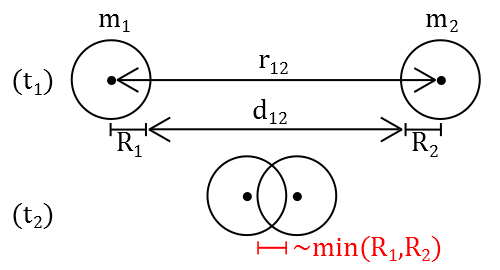
\includegraphics[width = 0.4\textwidth]{Figures/argument_for_epsilon.png}
\end{center}
\caption{Stars in motion}
\label{fig:afeps}
\end{wrapfigure}

Simulating two stars moving around each other in space, the method used is looking at them as point particles. This method is good to some extent, but it allows the stars to pass inside each other without this being a hindrance. In order to simulate that the stars are not in fact point particles, but have a radius R, as illustrated in \figref{fig:afeps}.  

To avoid this problem it is possible to introduce a small constant $\epsilon$ that acts as a smoothing function, giving a minimum distance between the stars. This prevents the stars from moving in to close to each other. Meaning that they now acts not like point particles but as objects with an extent in space. This epsilon changes \matref{eq:diffEq2} into 
\begin{align}
 \frac{\partial v}{\partial t} = -\frac{GM_2}{r^2 + \epsilon^2}
 \label{eq:SmoothingFct}
\end{align}





	\section{Generating Position, Mass and Velocity for Cluster Particles}
\label{Method:GeneratingPosMassVel}
\fxnote{write small intro}
\fxnote{in this section, we can introduce a generation of velocity, if we need that at some point}
\subsection{Gaussian Distributed Mass}
\fxnote{write here, what kind of distribution, we want!}

\begin{lstlisting}
void gaussian_mass_generator(vec (&mass), int number_of_particles)
{
  srand(time(NULL));
  for (int i = 0; i < number_of_particles; i++)
  {
  static int iset = 0;
  static double gset;
  double fac, rsq, v1, v2;
    do{
      v1 = 2.*((double) rand() / (RAND_MAX)) -1.0;
      v2 = 2.*((double) rand() / (RAND_MAX)) -1.0;
      rsq = v1*v1+v2*v2;
    } while (rsq >= 1.0 || rsq == 0.);
    fac = sqrt(-2.*log(rsq)/rsq);
    gset = v1*fac;
    iset = 1;
    mass(i) = v2*fac;
    mass(i) += 10;
  }
}
\end{lstlisting}

\begin{figure}[H]
\centering
	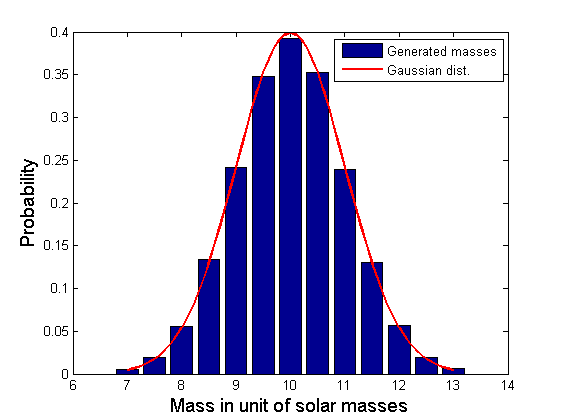
\includegraphics[width=0.7\linewidth]{Figures/random_mass_test.png}
\caption{
Histogram of the mass of 100,000 particles generated by the c++ code introduced \fxnote{where}. 
}
\label{fig:GaussianGeneratedMass}
\end{figure}
\fxnote{eq. include gaussian dist. in fig}

\subsection{Uniformly Distributed Position}
\fxnote{write here, what kind of distribution, we want!}

\begin{lstlisting}
void uniform_pos_generator(mat (&position), int N)
{
double pi=3.14159, c = 2*pi, R = 20;
vec phi(N), r(N), theta(N), x(N), y(N), v(N);

srand(time(NULL));

for (int i=0;i<N;i++){

        x(i) = ((double) rand() / (RAND_MAX)); //random numbers generated in the interval(0,1)
        y(i) = ((double) rand() / (RAND_MAX));
        v(i) = ((double) rand() / (RAND_MAX));
   }
for (int i=0;i<N;i++){
        phi(i)=c*x(i);
        r(i)=R*pow(y(i),1.0/3.0);
        theta(i)=acos(1.0-2.0*v(i));
        position(i,0)=r(i)*sin(theta(i))*cos(phi(i));
        position(i,1)=r(i)*sin(theta(i))*sin(phi(i));
        position(i,2)= r(i)*cos(theta(i));
   }
}
\end{lstlisting}

To test whether the generated positions within the sphere of radius $20$ ly, the density of particles in the cross-sectional area of each $x$-value is determined and plotted as a histogram in \figref{fig:UniformlyGeneratedPos} for $100,000$ particles with position generated by the introduced lines of code.  
The density of particles in the cross-sectional area of each $x$-value is found by dividing the total number of particles with that $x$-value with the cross-sectional area of the sphere in that $x$-value.
The cross-sectional area of the sphere in a specific area is found from a little trigonometry, by first considering that the radius of the circle that makes of the cross-sectional area in a point $x_i$ is given by $r_i = 20sin\theta_i$ ly.  
This yields that the area $A_i$ of the cross-sectional area, in ly, is given as
\begin{align}
	A_i = 400\pi sin^2 \theta_i =  400\pi (1 - cos^2 \theta)
\end{align}
in which the last equal sign stems from $1 = cos^2 \theta + sin^2 \theta$.
But $x_i = 20 cos \theta_i$ ly, giving
\begin{align}
	A_i = \pi (400 - x_i^2)
\end{align}
\begin{figure}[H]
\centering
	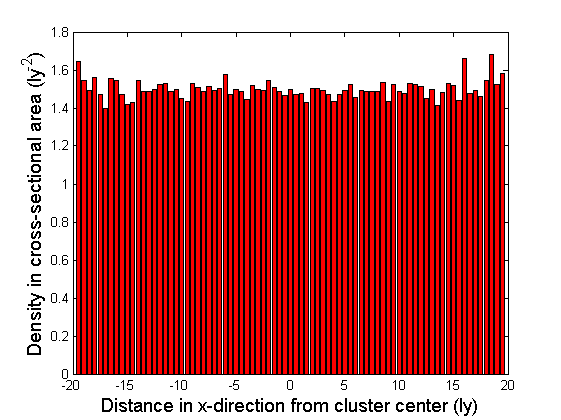
\includegraphics[width=0.7\linewidth]{Figures/random_uniform_position_test.png}
\caption{
Histogram of density of 100,000 particles with position generated by the code introduced in \fxnote{where??} as a function of the $x$-coordinate of the particles. The histogram is made with bins in the interval [$-19.5;19.5$] and a bin-size of $0.5$. The distance $x = \pm 20$ from the cluster center is not considered, since the cross-sectional area in that point is zero.
}
\label{fig:UniformlyGeneratedPos}
\end{figure}
	\section{Computing the Energy}
\label{sec:ComputingEnergy}
In order to test whether the energy is conserved, the initial energy of the system can be calculated and printed together with the final energy after a specific time interval.
According to the conservation of energy, these are equal. 

The total energy $E_{tot}$ of the system is found by summing up the potential energy $E_{pot}$ and kinetic energy $E_{kin}$ of the $N$ bodies that constitutes the system.
The total potential energy is calculated as 
\begin{align}
	E_{pot} = \sum _{1=0} ^N \sum _{j \neq i} \frac{m_i m_j}{r_{ij}}
\end{align}
in which $m_i$ and $m_j$ are the masses of the $i$'th and $j$'th body, respectively, $r_{ij} = | \v{r}_i - \v{r}_j |$ is the distance between the two bodies, and $G$ is the gravitational constant. 
The total kinetic energy of the system is calculated as 
\begin{align}
	E_{kin} = \frac{1}{2} \sum _{1=0} ^N m_i v_i ^2
\end{align}
with $v_i$ being the speed of the $i$'th particle calculated as 
$v_i = \sqrt{v_{ix}^2 +v_{iy}^2 +v_{iz}^2}$, and $m_i$ is the corresponding mass of that body. 

The c++ code for computing the total energy of the system is given here below.
When the kinetic energy is calculated, $v_i$ is not explicitly calculated. Instead $v_i^2$ is calculated to reduce the number of floating point operations. 
\begin{lstlisting}
for (int i=0; i<number_of_particles; i++){
	for (int k=0; k<3; k++){
    	kin_en(i) += v(i,k)*v(i,k);
    }
    kin_en(i) = 0.5*m(i)*kin_en(i);
    for (int j=0; j<number_of_particles; j++){
        if (j != i){
        	pot_en(i) += pow(distance_between_particles(i,j),-1.0)*m(j);
        }
    }
    pot_en(i) = pot_en(i)*G*m(i);
    tot_en(i) = kin_en(i)+pot_en(i);
}
\end{lstlisting}

	\chapter{Results and Discussion}
\label{chap:Results}
The starting point is solving the two body system, where Earth- and Sun-like forms the two bodies with masses $1\textrm{M}_{\odot}$ and $3\cdot 10^{-6} \textrm{M}_{\odot}$, respectively, for which $\textrm{M}_{\odot}$ is the solar mass. 
With the help of the Runge-Kutta method and the Velocity-Verlet method introduced in \secref{Newton2body3D}, the problem is solved both with a stationary Sun-like body relative to the frame of reference, and with both Earth and Sun moving relative to the coordinate system, with an initial velocity (0,0,0) and initial position an (1,1,1) for the Sun. 
For earth the initial position is assigned to be (2,1,1) and initial velocity (0,0.017,0). 

For an $N$ body system, the movement of the bodies with the evolution of time is estimated with the Velocity-Verlet method. 
From the result analysis the behaviour of the system is unfold.
\fxnote{ok, is this what we want to do?}

The results from running the codes described in \chapref{chap:method} for computing the blah blah blah ?? can be found in the GitHub folder  \url{https:/??}, together with the MatLab scripts for the plots presented in this chapter. \fxnote{fix these lines}

	\section{Stability of the 2-body System using Runge-Kutta and Velocity-Verlet}
\label{sec:stability2bodysystem}
The considered two-body system consists of an Earth-like body that orbits a Sun-like body at an initial distance of 1 AU. 
The initial velocity is chosen so that the orbital period of the Earth-like body is 365 days, and due to the choice of the initial position of the Earth-like body relative to the Sun-like body and the initial direction of the velocity of the Earth-like body, the orbit of the Earth-like body is purely in the $x-y$-plane.
Two cases are considered: the situation when the Sun is at rest compared to the frame of reference at all times, and the situation with both the Sun and the Earth moving relative to the frame of reference.
The chosen position and velocity vectors for the Earth and Sun in these two situations are shown in \tabref{tab:SunEarthMarsTest}. 
\begin{table}[H]
\centering
\caption{
Initial position and velocity for Earth and Sun in the Sun-Earth-like two-body system. 
F1 refers to the frame of reference at which the Sun is at rest in origo at all times, whilst F2 refers to the frame of reference in which both the Sun and the Earth moves relative to the coordinate axis. 
The mass of the Earth is given in solar masses, that is $\textrm{M}_E = 3.0\times 10^{-6} \textrm{M}_{\odot}$, and the gravitational constant is given is $2.96\cdot 10^{-4} \frac{\textrm{AU}^2}{\textrm{days}^2 \textrm{M}_{\odot}}$ (see \secref{sec:Conversion}).
}
\begin{center}
\begin{tabular}{ | c | c | c |  }
  \hline			
   &  $\v{r}_{initial}$ [AU] & $\v{v}_{initial}$ [AU/day]  
  \\ \hline
  Earth (F1) & $(1.0,0.0,0.0)$ & $(0.0,0.017,0.0)$
  \\ \hline
  Sun (F2) & $(1.0,1.0,1.0)$  & $(0.0,0.0,0.0)$ 
  \\ \hline
  Earth (F2)  & $(2.0,1.0,1.0)$ & $(0.0,0.017,0.0)$
  \\ \hline
\end{tabular}
\end{center}
\label{tab:SunEarthMarsTest}
\end{table}
\figref{fig:SunEarthMarsTest} shows the final distance between the two bodies as a function of time step length for the two situations: one in which sun is stationary relative to frame of reference and another in which sun is moving relative to the frame of reference. 
In both cases the final distance after 100 years is calculated between the Sun- and the Earth-like bodies and plotted as a function of length of time steps using both the fourth order Runga Kutta method and the Velocity-Verlet method. 
\begin{figure}[H]
\centering
\begin{minipage}{.5\textwidth}
  \centering
  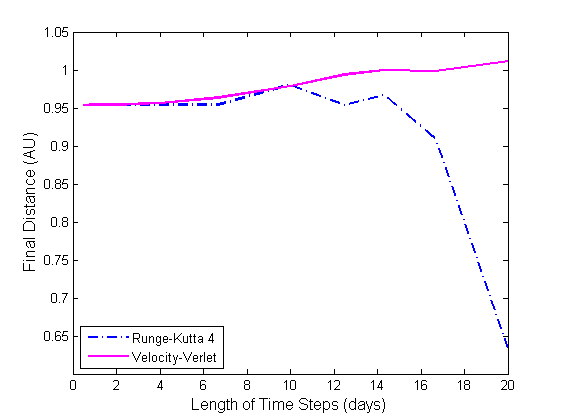
\includegraphics[width=1\linewidth]{Figures/Test_2body_system_earth.png}
\end{minipage}%
\begin{minipage}{.5\textwidth}
  \centering
  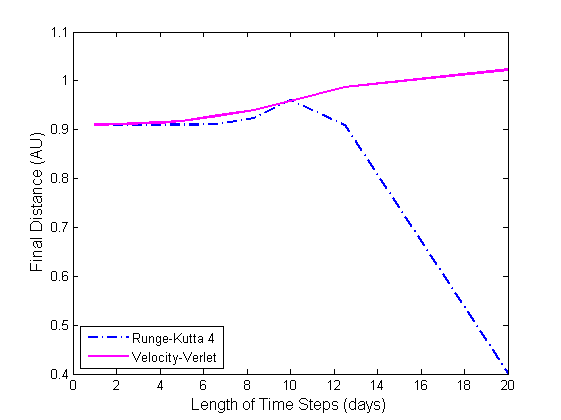
\includegraphics[width=1\linewidth]{Figures/Test_2body_system_earth_sun.png}
\end{minipage}
\caption{
Distance between bodies after 100 years as a function of time step length for the Earth-Sun-like two-body system using both the forth order Runge-Kutta method and the Velocity-Verlet method. 
The leftmost plot do not allow for Sun motion relative to the frame of reference, whilst the rightmost allows for movement of both the Earth and the Sun relative to the frame of reference.
}
\label{fig:SunEarthMarsTest}
\end{figure}
The result using the Velocity-Verlet method shows a gradual increase in the final distance between the two bodies after 100 years, as the length of time steps increases, whereas the final distance after 100 years gained by the fourth order Runga-Kutta method shows fluctuations for shorter time step lengths, which is slightly more when sun is stationary relative to the frame of reference.
As time step length reaches about 10 days, the distance, determined by the Runge-Kutta method, between the two bodies decreases, and the final distance after 100 years between the Earth-like body and the Sun-like body starts varying a lot with a change in time step length, meaning that the Runge-Kutta method is very unstable for large time steps, greater than approximately 10 days for this situation.
However, both the Velocity-Verlet and forth order Runge-Kutta method seems to have stabilized for time steps smaller than or equal to 5 days, both for the situation with a stationary Sun and for the situation with both the Sun and Earth moving relative to the coordinate system.
Hence, the time step length of 5 days is used to study the stability of the two methods for long time periods in \figref{fig:SunEarthMarsTest2}.
\begin{figure}[H]
\centering
\begin{minipage}{.5\textwidth}
  \centering
  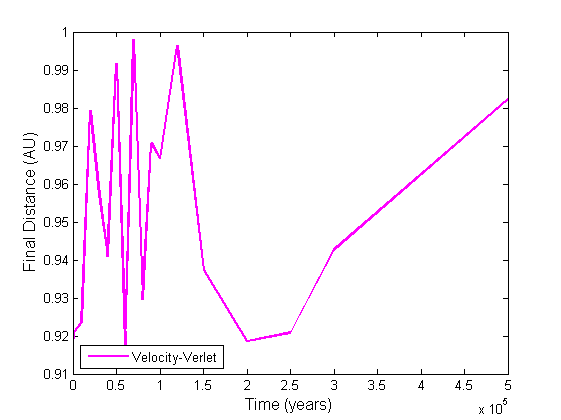
\includegraphics[width=1\linewidth]{Figures/test_distance_time_VV.png}
\end{minipage}%
\begin{minipage}{.5\textwidth}
  \centering
  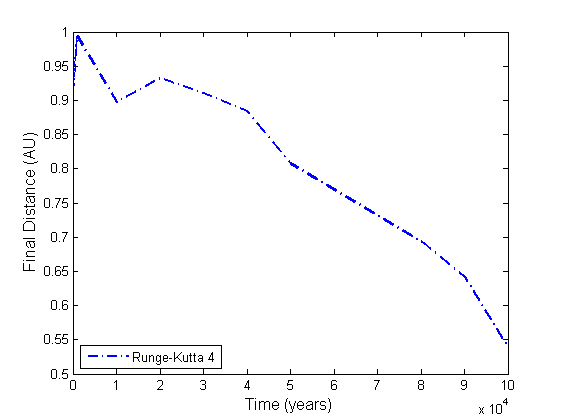
\includegraphics[width=1\linewidth]{Figures/test_distance_time_RK4.png}
\end{minipage}
\caption{
The final distance as a function of time with a time step length of 5 days for both the Velocity-Verlet and Runge-Kutta method with both the Earth and Sun moving relative to the frame of reference.
After $2.5\times 10^4$ years, the Earth continuously moves towards the Sun, in the Runge-Kutta method, whilst the distance between the Earth and Sun still fluctuates between 0.92 AU and 1 AU for the Velocity-Verlet method after $5\times 10^5$ years.  
}
\label{fig:SunEarthMarsTest2}
\end{figure}
When allowing for motion of both the Earth and the Sun relative to the frame of reference, both the Velocity-Verlet method and the forth order Runge-Kutta method show that the distance between the Earth-like body and the Sun-like body will fluctuate with time, which seems reasonable from the fact that Earth's orbit around the Sun is not circular but elliptical. 
From the Runge-Kutta method it is found that after approximately $2.5\times 10^4$ years the Earth will start moving rapidly towards the Sun, and after $10^5$ years the distance between the Sun-like object and the Earth-like object is only around $0.55$ AU. This is, however, not seen in the Velocity-Verlet method.
In the real solar system, the orbit of the Earth is in addition to the gravitational pull from the Sun also affected by the presence of the other planets. 
In the absence of these remaining planets and other objects in the solar system, the movement of the Earth-like object considered in this two-body system will, obviously, be different from the orbit known from astrophysics.
However, it is estimated that the absence of other objects in the solar system, will not cause this rapid motion of Earth and Sun towards each other after only in the order of $10,000$ years, and hence it is concluded that the rapid motion seen in the rightmost figure of \figref{fig:SunEarthMarsTest2} is due to instabilities in the fourth order Runge-Kutta method presented in \secref{sec:methodRK4}, yielding a greater stability in the Velocity-Verlet method than in the Runge-Kutta method for solving this two-body problem.

The table below shows the respective computational times for the fourth order Runge-Kutta method and the Velocity-Verlet method for computing the final position after 1 year using different time step length. 
\begin{table}[H]
\centering
\caption{
Computational time for the fourth order Runge-Kutta method and the Velocity-Verlet method for different time steps during 1 year.
}
\begin{center}
\begin{tabular}{ | c | c | c | }
  \hline			
  \# time steps  & Comp. time RK4 & Comp. time VV  
  \\ \hline
  1 & 6 & 2
  \\ \hline
  10 & 25 & 8
  \\ \hline
  $10^4$ & $8.4\times 10^3$ & $4.6\times 10^3$
  \\ \hline
  $10^6$ & $8.0\times 10^5$ & $3.6\times 10^5$
  \\ \hline
\end{tabular}
\end{center}
\label{tab:SunEarthMarsTest2}
\end{table}
From the table it is evident that the computational time of both the fourth order Runge-Kutta method and the Velocity-Verlet method is more or less proportional to the number of time steps.
Furthermore, the Velocity-Verlet method seems to be faster than the Runge-Kutta mthos for all investigated number of time steps. 
Together with the grater stability of the Velocity-Verlet method than the Runge-Kutta method, this yields that it is an advantage to use the Velocity-Verlet method to study this two-body system.  
	\section{Testing Runge-Kutta and Velocity-Verlet for Sun-Earth-Mars System}
\label{sec:SunEarthMarsTest}

\begin{table}[H]
\centering
\caption{Mass, initial position and initial velocity of Sun, Earth and Mars when running the Runge-Kutta 4 algorithm for this three-body problem.
The Earth and Mars are set to orbit in the $x-y$-plane at $z=1$ AU with the distance 1 AU and 1.5 AU to the Sun, respectively, which is not physically true. However, this initialization of position and velocity is reasonable to illustrate the validity of the Runge-Kutta method and Velocity-Verlet method presented in \secref{Newton2body3D}.
}
\begin{center}
\begin{tabular}{ | c | c | c | c |  }
  \hline			
   & mass [$M_{\odot}$] &  $\v{r}_{initial}$ [AU] & $\v{v}_{initial}$ [AU/day]  
  \\ \hline
  Sun & $1.0$ & $(1.0,1.0,1.0)$  & $(0.0,0.0,0.0)$ 
  \\ \hline
  Earth & $3.0\times 10^{-6}$ & $(2.0,1.0,1.0)$ & $(0.0,0.017,0.0)$
  \\ \hline
  Mars & $3.2\times 10^{-7}$ & $(-0.5,1.0,1.0)$  & $(0.0,0.014,0.0)$
  \\ \hline
\end{tabular}
\end{center}
\label{tab:SunEarthMarsTest}
\end{table}

    
\begin{figure}[H]
\centering
\begin{minipage}{.5\textwidth}
  \centering
  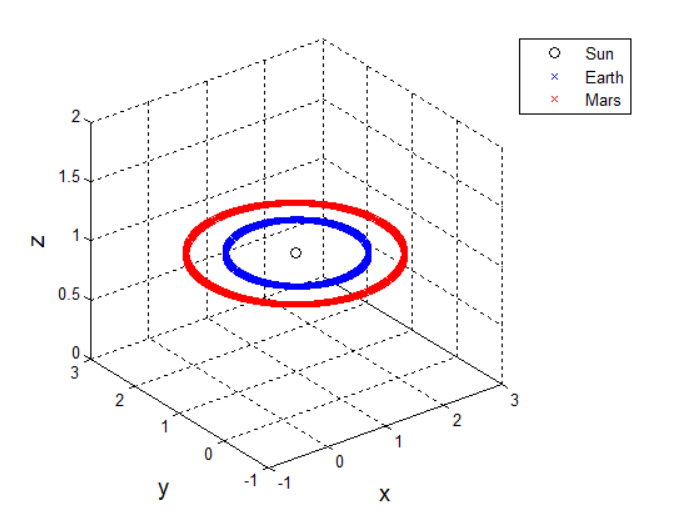
\includegraphics[width=1\linewidth]{Figures/sun_earth_mars_test_RK4.png}
\end{minipage}%
\begin{minipage}{.5\textwidth}
  \centering
  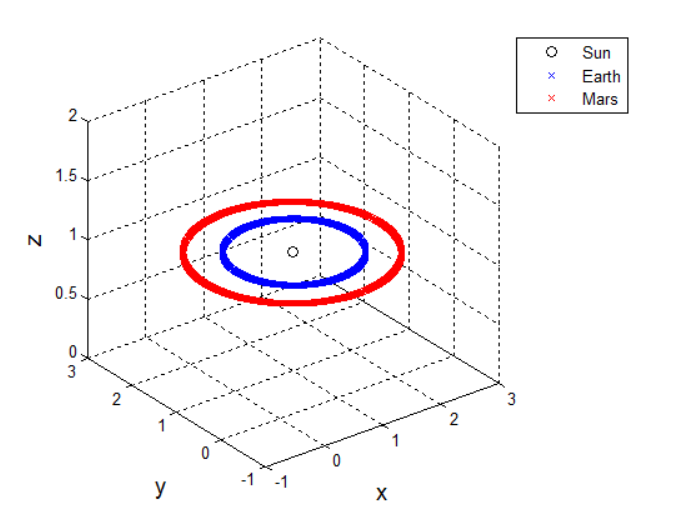
\includegraphics[width=1\linewidth]{Figures/sun_earth_mars_test_VV.png}
\end{minipage}
\caption{
Time evolution of the simplified system of Sun-Earth-Mars over a time period of 20 years using Runge-Kutta (leftmost) and Velocity-Verlet (rightmost) method with a time step length of 1 day.
The masses, initial positions, and initial velocities of the three objects are given in \tabref{tab:SunEarthMarsTest}.
}
\label{fig:SunEarthMarsTest}
\end{figure}

Calculating the initial and final energy of the Sun-Earth-Mars system according to the source code presented en \secref{sec:ComputingEnergy}, gives the following table for different time periods with step length of 1 day.

\begin{table}[H]
\centering
\caption{The final energy after different time periods computed by both the first order Runge-Kutta method and the Velocity-Verlet method for the Sun-Earth-Mars-like system with initial energy of $2.37\times 10^{-9} \text{M}_{\odot} \text{AU}^2 /\text{days}^2$ .
}
\begin{center}
\begin{tabular}{ | c | c | c |  }
  \hline	
  Time period (years) & Final energy (RK4) & Final energy (VV)
  \\ \hline		
  1  & $2.37\times 10^{-9}$ & $2.37\times 10^{-9}$
  \\ \hline
  10  & $2.47\times 10^{-9}$ & $2.47\times 10^{-9}$
  \\ \hline
  100  & $2.50\times 10^{-9}$ & $2.50\times 10^{-9}$
  \\ \hline
  1000 & $2.38\times 10^{-9}$  & $2.38\times 10^{-9}$ 
  \\ \hline
\end{tabular}
\end{center}
\label{tab:SunEarthMarsTest_energy_conservation}
\end{table}
It seems alarming that the final energy if greater than the initial energy for both the fourth order Runge-Kutta method and the Velocity-Verlet method. 
However, with the precision of the constants, e.g. the gravitational constant $G=2.96\times 10^{-4} \text{AU}^3 / \text{days}^2 \cdot \text{M}_{\odot}$, and the time steps, it is conclusive to say that the programmed code for this N-body problem  
	\section{Time Step Length in the N-body Problem}
\label{sec:TimeStepLengthNbody}
When estimating the time step length required to study the evolution of the star cluster consisting of $N=100$ particles initially uniformly distributed in a sphere of radius $20$ ly with normal distributed masses with mean $10{\textrm{M}}_{\odot}$, the initial and final distribution of particles in the radial direction for a finite time period is studied for different time step lengths. 
The time period, considered, is chosen to be of the order of the characteristic time $\tau _{crunch}$, given in \matref{eq:t_crunch}.
$\tau _{crunch}$ is the finite time at which the system with $N \rightarrow \infty$ particles with no or low initial velocity collapses into a singularity. \fxnote{ref!}
\begin{align}
	\tau _{crunch} = \sqrt{\frac{3\pi}{32G\rho_0}}
	\label{eq:t_crunch}
\end{align}
With the units light years, years and solar masses ${\textrm{M}}_{\odot}$, the value of the gravitational constant is, according to \secref{sec:Conversion}, $G = 1.536\cdot 10^{-13} \textrm{ly}^3 / \textrm{yr}^2 {\textrm{M}}_{\odot}$, whilst the mass density of $N=100$ particles with a mean mass of $10 {\textrm{M}}_{\odot}$ within the sphere of radius $20 \text{ly}$ is 
$\rho_0 = 10 {\textrm{M}}_{\odot} / (4/3 \pi (20 \text{ly})^2)$, yielding that the $\tau _{crunch}$ becomes
\begin{align}
	\tau _{crunch} = \sqrt{\frac{12\pi^2\cdot 20^3}{32\cdot 1.536\cdot 10^{-13}}\cdot 10\cdot 3} \text{ yr} 
	\approx 8.0\times 10^7 \text{ yr}
\end{align}
The histograms in \figref{fig:histograms_VV_diff_time_step} and \ref{fig:histograms_RK4_diff_time_step} show the initial and final radial position of 100 particles in a sphere of radius $20$ ly, initially at rest, interacting only through the Newtonian force between all particles, after $10^7$ years with different step lengths. 
The masses and initial position of the 100 particles are generated by the functions given in \secref{Method:GeneratingPosMassVel}.
the final positions given in the histograms of \figref{fig:histograms_VV_diff_time_step} are computed with the Velocity-Verlet method for N bodies, whilst the final positions given in the histograms of \figref{fig:histograms_RK4_diff_time_step} are computed with the fourth order Runge-Kutta method for N bodies.
\begin{figure}[H]
\centering
\begin{minipage}{.5\textwidth}
  \centering
  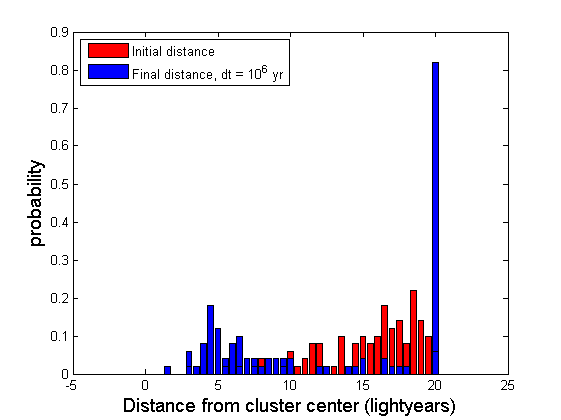
\includegraphics[width=1\linewidth]{Figures/graphs_VV/pos1_VV.png}
\end{minipage}%
\begin{minipage}{.5\textwidth}
  \centering
  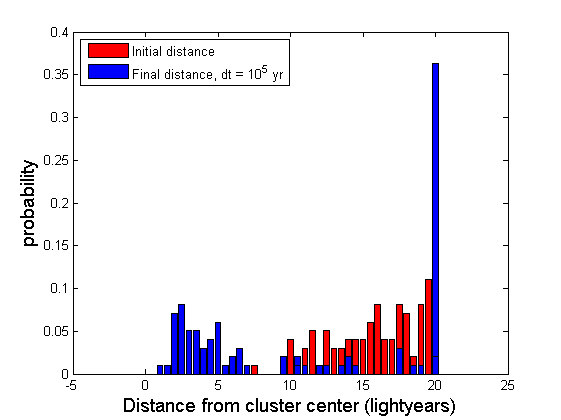
\includegraphics[width=1\linewidth]{Figures/graphs_VV/pos2_VV.png}
\end{minipage}
\begin{minipage}{.5\textwidth}
  \centering
  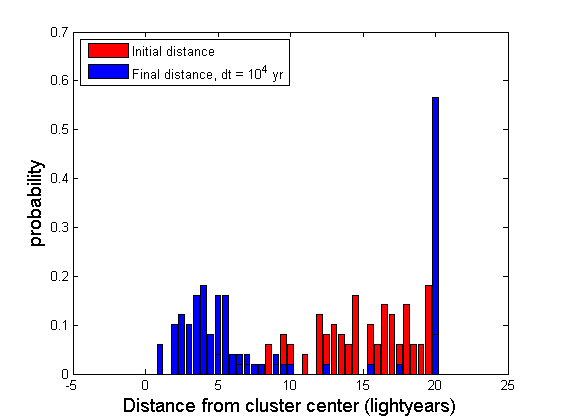
\includegraphics[width=1\linewidth]{Figures/graphs_VV/pos3_VV.png}
\end{minipage}%
\begin{minipage}{.5\textwidth}
  \centering
  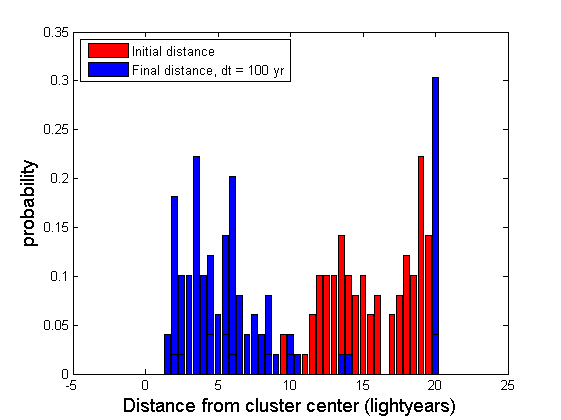
\includegraphics[width=1\linewidth]{Figures/graphs_VV/pos5_VV.png}
\end{minipage}
\caption{
Initial and final position position over a time period of $10^7$ years for 100 particles in a sphere of radius $20$ ly computed by the Velocity-Verlet method, for different time step lengths $dt$.
The masses of the particles are normal distributed around $10{\textrm{M}}_{\odot}$ with a standard deviation of $1{\textrm{M}}_{\odot}$, whilst the initial positions are computed from an initial uniform density within the sphere.
The depicted particle probability at the distance $r=20$ ly correspond to particles that are actually at around $20$ ly away from the cluster center after $10^7$ years, but it also accounts for the particles that has escaped the cluster, that is $R>20$ ly.
}
\label{fig:histograms_VV_diff_time_step}
\end{figure}
By comparing the four histograms in \figref{fig:histograms_VV_diff_time_step} for different time step lengths, in seems that the final radial distribution of the particles after $10^7$ years consists of three distinct features. Close to the center, at a distance smaller that $5-10$ ly, a high density seems to appear. 
In addition a great part of the particles seem to be ejected from the cluster. 
This is seen by the high probability bar at a distance $R=20$ ly from the cluster center. This bar represents both particles at the edge of the cluster and particles that have been ejected from the cluster. 
For long time steps, this ejection seems to be greater than for short time steps.
That is, for a step length of $dt = 10^6$ yr, the amount of particles that has been ejected from the cluster after $10^7$ yr is roughly $40 \%$, whilst the amount of ejected particles with a step length of $dt = 100$ years is only around $15 \%$.
This is similar to the result gained in \secref{sec:stability2bodysystem}, where the distance between the bodies after 100 years in the Sun-Earth-like system was computed to be greater for larger time step lengths than for short time step lengths for the Velocity-Verlet method, as well, as seen in \figref{fig:SunEarthDistanceAfter100yr}. 
The third feature of the histograms in \figref{fig:histograms_VV_diff_time_step} is the small density of particles at more than $10$ ly away from the cluster center.
All of the histograms with different time step lengths show these same features, apart from the number of ejected particles, which vary rapidly with decreased step length. 
\begin{figure}[H]
\centering
\begin{minipage}{.5\textwidth}
  \centering
  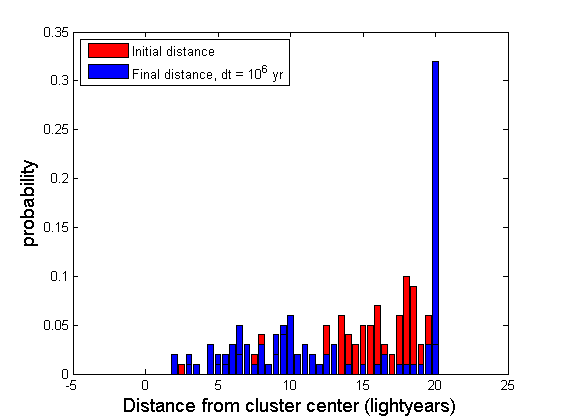
\includegraphics[width=1\linewidth]{Figures/graphs_RK4/pos6.png}
\end{minipage}%
\begin{minipage}{.5\textwidth}
  \centering
  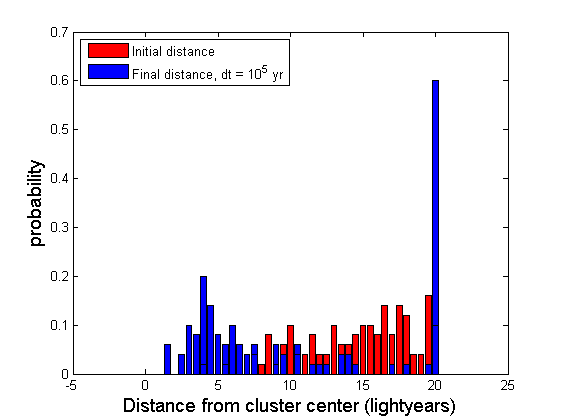
\includegraphics[width=1\linewidth]{Figures/graphs_RK4/pos5.png}
\end{minipage}
\begin{minipage}{.5\textwidth}
  \centering
  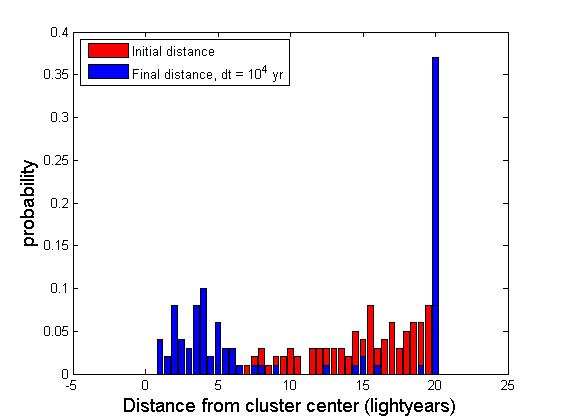
\includegraphics[width=1\linewidth]{Figures/graphs_RK4/pos4.png}
\end{minipage}%
\begin{minipage}{.5\textwidth}
  \centering
  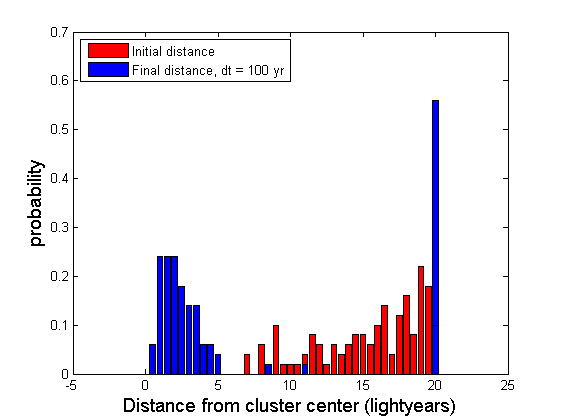
\includegraphics[width=1\linewidth]{Figures/graphs_RK4/pos9.png}
\end{minipage}
\caption{
Initial and final position position over a time period of $10^7$ years for 100 particles in a sphere of radius $20$ ly computed by the Fourth order Runge-Kutta method, for different time step lengths $dt$.
The masses of the particles are normal distributed around $10{\textrm{M}}_{\odot}$ with a standard deviation of $1{\textrm{M}}_{\odot}$, whilst the initial positions are computed from an initial uniform density within the sphere.
The depicted particle probability at the distance $r=20$ ly correspond to particles that are actually at around $20$ ly away from the cluster center after $10^7$ years, but it also accounts for the particles that has escaped the cluster, that is $R>20$ ly.
}
\label{fig:histograms_RK4_diff_time_step}
\end{figure}
\fxnote{is it ok that I have just copy-pasted caption??}

As for the radial distribution after $10^7$ years computed by the Velocity-Verlet method, the final distribution shown in \figref{fig:histograms_RK4_diff_time_step}, computed by the fourth order Runge-Kutta method, show the three features: high density close to the center, low density at a more than $10$ ly from the center, and an ejection of particles from the cluster.
However, for long time steps, that is $dt = 10^6$ yr, these features are not as distinct, yielding that this step length is too long for the Runge-Kutta method. 
Unlike the Velocity-Verlet method, the amount of particles that are ejected from the cluster using the Runge-Kutta method seems, however, to be stable for all depicted step lengths at around $30 \%$. 

In the two particle case the Velocity-Verlet method seemed like it was the most stable method over time. Looking at the N particle case the Velocity-Verlet is more dependent of the choice of time step, whilst the Runge-Kutta 4 method is more stable towards the change in time-step. This might have a lot to say for the stability of the system and the computational time. Therefore the Runge-Kutta 4 method seems like the better choice when looking at times greater than $\tau_{crunch}$. 



After finding the positions of the particles after a time in the order of a $\tau_{crunch}$, the star cluster have not collapsed into a mass in the middle. Therefore using $\tau_{crunch}$ as a unit of time to study the further behaviour is a natural conclusion. For this to work the gravitational constant has to be transformed into units that fits and for the N particle case. Using \matref{eq:t_crunch} it's possible to find the gravitational constant as a function of particles N.  
\begin{align}
G = 986.96 \frac{1}{N} \frac{\textrm{ly}^3}{\tau_{crunch}^2\textrm{m}_{mean}}
\end{align}

Now when looking at timescales larger than $\tau_{crunch}$, the time steps have to be calculated from the new unit of time $\tau_{crunch}$. From the histograms in \figref{fig:histograms_RK4_diff_time_step} the best time step length to choose is $10^5$ years. If this is then transformed into the new time scale it is
\begin{align*}
dt = 10^{-3} \tau_{crunch}
\end{align*}

	\section{Stability and Equilibrium of $N=100$ System}
\label{sec:StabilityAndEquilibrium}
From the histograms in \figref{fig:histograms_RK4_diff_time_step}, it is expected that the extend of the cluster will vary with time. 
In the histograms of \figref{fig:StabilityEquilibriumHistogram}, the final position of 100 uniformly distributed particles with Gaussian distributed masses, as previous, is computed with the fourth order Runge-Kutta method after $1\tau_{crunch}$ and $4\tau_{crunch}$ with the same step length, $dt = 10^{-3} \tau_{crunch}$. 
Similar histograms are made for the final position after $0.5\tau_{crunch}$, $1.5\tau_{crunch}$, $2\tau_{crunch}$, $2.5\tau_{crunch}$, $3\tau_{crunch}$, as well. 
However, these histograms are not explicitly shown in this work. 
\begin{figure}[H]
\centering
\begin{minipage}{.5\textwidth}
  \centering
  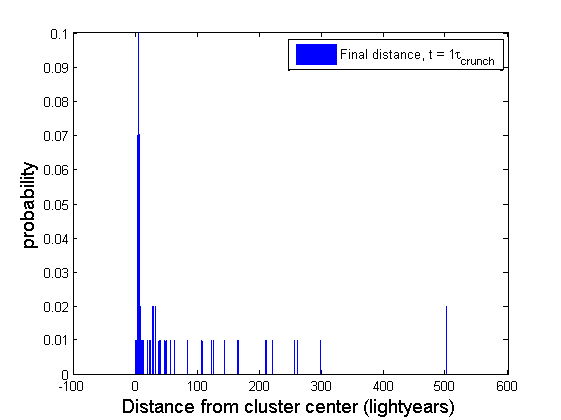
\includegraphics[width=1\linewidth]{Figures/stability/RK4_stability_1t.png}
\end{minipage}%
\begin{minipage}{.5\textwidth}
  \centering
  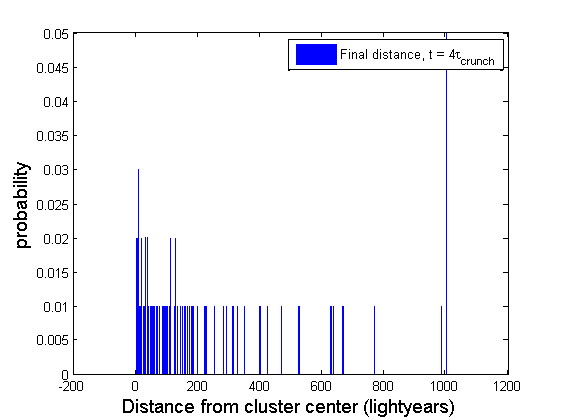
\includegraphics[width=1\linewidth]{Figures/stability/RK4_stability_4t_2_zoom.png}
\end{minipage}
\caption{
Final radial position of 100 particles after $1\tau_{crunch}$ and $4\tau_{crunch}$ with a step length of $10^{-3} \tau_{crunch}$.
The "high" densities at 500 ly and 1000 ly represent particles further away from the cluster center than 500 ly or 1000 ly, respectively.
The extend of the cluster is here defined as the first particle than has a distance of 100 ly to the next particle further from the cluster center. 
Hence after $1\tau_{crunch}$, the extend of the cluster is 166 ly, whilst after $4\tau_{crunch}$, the cluster extend is 525 ly.
}
\label{fig:StabilityEquilibriumHistogram}
\end{figure}
The knowledge of the cluster extend as a function of time gained from \figref{fig:StabilityEquilibriumHistogram} is plotted in the figure below. 
The plotted data show reaching of an equilibrium after approximately $2\tau_{crunch}$.
Another argument for reaching the equilibrium after about $2\tau_{crunch}$ is the number of particles within a sphere of radius of $10$ ly, which is inspired by the great density of particles within this sphere compared to density outside this sphere after $10^7$ years, shown in the histograms of \figref{fig:histograms_RK4_diff_time_step}. 

%\begin{figure}[H]
%\centering
%	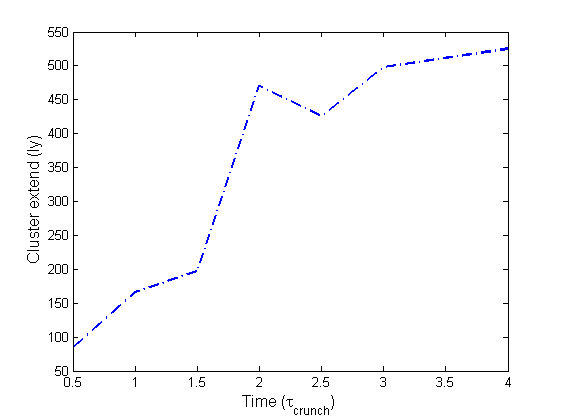
\includegraphics[width=0.6\linewidth]{Figures/Stability_cluster_extend_time_dependence.png}
%\caption{
%Plot of the cluster extend as a function of the final time. The cluster extend is determined from histograms similar to the ones shown in \figref{fig:StabilityEquilibriumHistogram}.
%}
%\label{fig:StailityEquilibriumLineGraph}
%\end{figure}
\begin{minipage}{\textwidth}
  \begin{minipage}[c]{.5\textwidth}
    \centering
    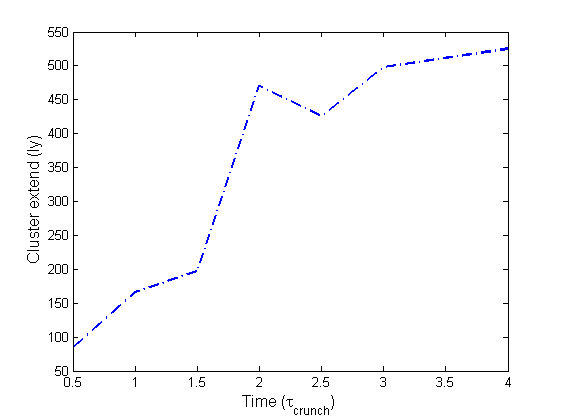
\includegraphics[width=1\linewidth]{Figures/Stability_cluster_extend_time_dependence.png}
    \captionof{figure}{Plot of the cluster extend as a function of the final time. The cluster extend is determined from histograms similar to the ones shown in \figref{fig:StabilityEquilibriumHistogram}.}
    \label{fig:StailityEquilibriumLineGraph}
  \end{minipage}
  \hfill
  \begin{minipage}[c]{.5\textwidth}
    \centering
    \begin{tabular}{|c|c|}\hline
      	Time [$\tau_{crunch}$] & \# particles \\ \hline
        0.5 & 31 \\
        1 & 62 \\
        1.5 & 38 \\
        2 & 23 \\
        2.5 & 17 \\
        3 & 6 \\ 
        4 & 12
        \\ \hline
      \end{tabular}
      \captionof{table}{Number of particles within a sphere of radius $10$ ly after various times.}
    \end{minipage}
\end{minipage}

	\section{Energy of the $N$-body Runge-Kutta Method}
\label{sec:EnergyRK4}

\fxnote{write here that we take minus solution}

In the table below, the initial energies, final energies and energy losses are shown together with the percentage of kinetic energy of the total final energy for different number of particles $N$ after a time period of $2\tau_{crunch}$. 
A clear tendency in the energy loss of about $32 \%$ for all considered sizes of systems. 
Furthermore after the time period of $2\tau_{crunch}$, the kinetic energy constitutes to $40 \% - 50\%$ of the total energy for all the system sizes. 
This, of course, yields a drastic decrease en the potential energy of the system, since the initial kinetic energy is set to zero. 


\begin{table}[H]
\centering
    \begin{tabular}{|c|c|c|c|c|}\hline
      	N & Initial Energy & Final energy & Energy loss (\%) & $E_{kin}$ of $E_{final}$  
      	\\ \hline
        10 & 62384 & 39075 & 37.4 & 40.3
        \\ \hline
        20 & 107840 & 73086 & 32.2 & 47.6
        \\ \hline
        30 & 180199 & 119402 & 33.7 & 49.1
        \\ \hline
        40 & 212556 & 146758 & 31.0 & 44.8
        \\ \hline
        50 & 276332 & 187268 & 33.2 & 47.6
        \\ \hline
        60 & 360979 & 246919 & 31.6 & 46.2
        \\ \hline
        70 & 407283 & 275201 & 32.4 & 48.0
        \\ \hline
        80 & 446740 & 307724 & 31.1 & 45.2
        \\ \hline
        90 & 544320 & 364427 & 33.0 & 49.4
        \\ \hline
        100 & 599065 & 409111 & 31.7 & 46.4
        \\ \hline
      \end{tabular}
      \captionof{table}{
      Initial energy, final energy, total energy loss and the percentage of $E_{kin}$ of the total final energy after a time period of $2\tau_{crunch}$ with a step length of $10^{-3}\tau_{crunch}$, and $G = 986.96/N \textrm{ ly}^3/\tau_{crunch}^2\textrm{m}_{mean}$, for different number of particles $N$.
      }
      \label{EnergyRK4differentN}
\end{table}

\begin{table}[H]
\centering
    \begin{tabular}{|c|c|c|c|c|}\hline
      	$t_final$ [$\tau_{crunch}$] & Initial Energy & Final energy & Energy loss (\%) & $E_{kin}$ of $E_{final}$  
      	\\ \hline
        2 & 276332 & 187268 & 32.2 & 47.6
        \\ \hline
        3 & 268708 & 170423 & 36.6 & 57.7
        \\ \hline
        4 & 302486 & 177473 & 41.3 & 70.4
        \\ \hline
      \end{tabular}
      \captionof{table}{
      Initial energy, final energy, total energy loss and the percentage of $E_{kin}$ of the total final energy for a system of $50$ particles and with $G = 986.96/N \textrm{ ly}^3/\tau_{crunch}^2\textrm{m}_{mean}$ after different time periods with a step length of $10^{-3}\tau_{crunch}$.
      }
      \label{EnergyRK4differenttime}
\end{table}

\fxnote{this looks like we have not reached equilibrium at this point!}
	\section{Distribution of Potential and Kinetic Energy of Bound Particles after a Finite Time}
\label{sec:DistributionPotKinEnBound}
The virial theorem states the following relation for the kinetic energy $E_{kin}$ and potential energy $E_{pot}$ of a bound gravitational system in equilibrium. 
\begin{align}
	2\left< E_{kin} \right> = - \left< E_{pot} \right>
	\label{eq:ViralTheorem}
\end{align}
$\left< E_{kin} \right>$ and $\left< E_{pot} \right>$ represents the time average of the kinetic and potential energy, respectively, but by the ergodic hypothesis, this can be made the ensamble average \cite{Project5_CompPhys}. 

To study whether the virial theorem of \matref{eq:ViralTheorem} is fulfilled with the computed algorithms, the final kinetic and potential energy of the bound particles of a system initially consisting of 70 particles after a time period of $\tau_{crunch}$.
It is expected that the fraction of the mean of the kinetic energy and the mean of the potential energy will be close to $-2$, even though it in \secref{sec:StabilityAndEquilibrium} is found that the equilibrium is not reached before than after a time period of $2\tau_{crunch}$. 

In addition, to get rid of some of the numerical instabilities, a smoothing function, as argued for in \secref{sec:argumentforepsilon}, is introduced.
To check the consistency with the virial theorem of the fourth order Runge-Kutta method when including the smoothing function, similar histograms for the distribution of the kinetic energy and potential energy after a finite time period as shown in \figref{fig:DistributionPotKinEnBoundHistograms} is generated to determine the mean of the kinetic energy and potential energy.
The bound particles are found by the same argument as in \fxnote{ref to magnus-sec} that a particle is bound if the total energy of that particle is negative, that is the particle is bound if the absolute value of the potential energy is greater than the absolute value of the kinetic energy.
\begin{figure}[H]
\centering
\begin{minipage}{.5\textwidth}
  \centering
  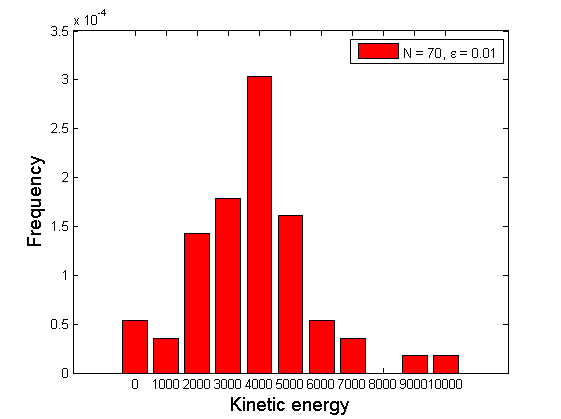
\includegraphics[width=1\linewidth]{Figures/Histograms_including_epsilon/N_70_e_n3_kin.png}
\end{minipage}%
\begin{minipage}{.5\textwidth}
  \centering
  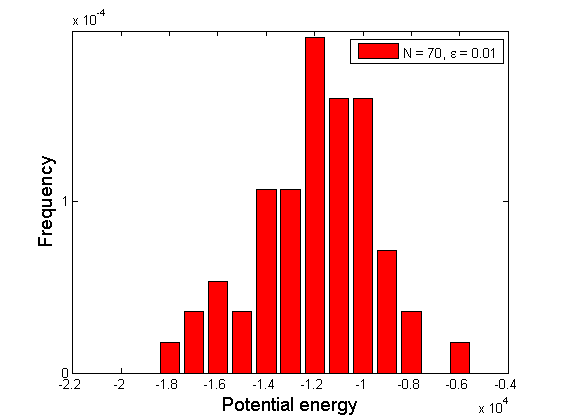
\includegraphics[width=1\linewidth]{Figures/Histograms_including_epsilon/N_70_e_n3_pot.png}
\end{minipage}
\caption{
	Distribution of the kinetic and potential energy of bound particles in the star cluster after a time period of $1\tau_{crunch}$ with a step length of $1\times 10^{-4} \tau_{crunch}$ and $\epsilon = 1\times 10^{-2} \text{ ly}$ for 70 particles with normal distributed masses, uniformly distributed within a sphere generated by the functions presented in \secref{Method:GeneratingPosMassVel}. 
}
\label{fig:DistributionPotKinEnBoundHistograms}
\end{figure}
The kinetic and the potential energy of the bound particles seem to follow a more or less uniform distribution after a finite time period. 
This is also seen when computing histograms for different values of $\epsilon$. 
The mean of these distributions for the kinetic energy and potential energy after are shown in the table below for various values of $\epsilon$. 

\begin{table}[H]
\centering
\begin{tabular}{|c|c|c|c|c|}
\hline
$\epsilon$ (ly)  & $\left< E_{kin} \right>$ & $\left< E_{pot} \right>$ & $\left< E_{pot} \right>$/$\left< E_{kin} \right>$ \\
\hline
0 & 952.0 & -2409 & -2.53	
\\ \hline
0.1 & 4036 & -7886 & -1.95
\\ \hline
$10^{-2}$ & 1119 & -2846 & -2.54
\\ \hline
$10^{-3}$ & 2548 & -4860 & -1.91
\\ \hline
$10^{-4}$ & 2531 & -4489 & -1.77
\\ \hline
$10^{-5}$ & 2129 & -3677 & -1.73
\\ \hline
$10^{-6}$ & 567.5 & -1774 & -3.13
\\ \hline
$10^{-7}$ & 1333 & -2444 & -1.83
\\ \hline
$10^{-8}$ & 1368 & -2635 & -1.93
\\ \hline
\end{tabular}
\caption{
Mean of kinetic energy and potential energy for bound particles after a time period of $3\tau_{crunch}$ with a step length of $10^{-4} \tau_{crunch}$ for a star cluster with initially 70 particles uniformly distributed in a sphere of radius $20\text{R}_{\odot}$.
The computed potential energy is divided by two, since in the computation the potential energy is doubled when summing up for all particles. 
}
\label{tab:DistributionPotKinEnBound}
\end{table}
From \tabref{tab:DistributionPotKinEnBound} it is seen that for no values of $\epsilon$, the virial theorem is fulfilled. 
However, the fraction $\left< E_{pot} \right>$/$\left< E_{kin} \right>$ approaches the value $-2$, when $\epsilon$ is introduced for all values except $\epsilon = 10^{-6}$.
The fraction of the energies is in the figure below plotted as a function of $\epsilon$, and it is seen from the figure, as well from \tabref{tab:DistributionPotKinEnBound} that most of the choices of $\epsilon$ will be an improvement of the result compared having $\epsilon = 0$, according to the virial theorem.
Since $10^{-7} \text{ly}$ corresponds to $1.36\text{R}_{\odot}$ this is chosen as the optimal $\epsilon$, due to the fact that is has the physical meaning of being similar to what one can expect the radius of the considered particles to be.
\begin{figure}[H]
\centering
	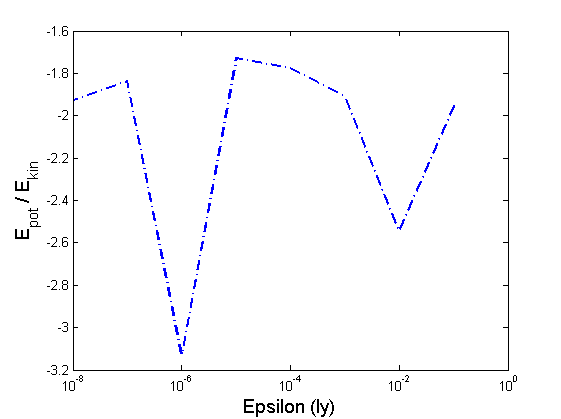
\includegraphics[width=0.6\linewidth]{Figures/epsilon_frac.png}
\caption{
The value of the energy fraction $\left< E_{pot} \right>$/$\left< E_{kin} \right>$, that according to the virial theorem should equal $-2$, as a function of $\epsilon$ introduced in \matref{eq:SmoothingFct}.
}
\label{fig:epsilonfrac}
\end{figure}
The histograms in \figref{fig:DistributionPotKinEnBoundHistograms2} below show the distribution of the kinetic energy and potential energy of the bound particles after a time period of $3\tau_{crunch}$, hence after reached equilibrium. 
The distribution of the energies of the bound particles seems no longer to be Gaussian as was seen for a time period of $1\tau_{crunch}$ in \figref{fig:DistributionPotKinEnBoundHistograms}.
\begin{figure}[H]
\centering
\begin{minipage}{.5\textwidth}
  \centering
  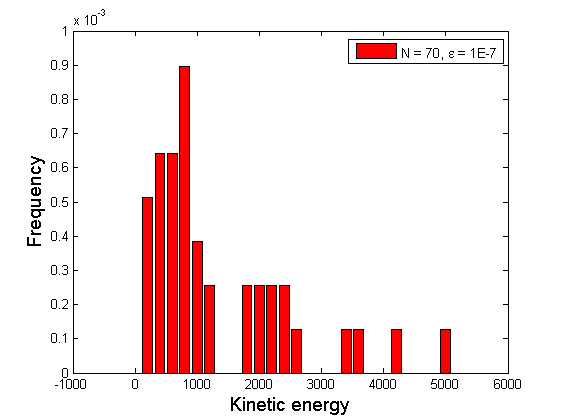
\includegraphics[width=1\linewidth]{Figures/epsilon7_kin.png}
\end{minipage}%
\begin{minipage}{.5\textwidth}
  \centering
  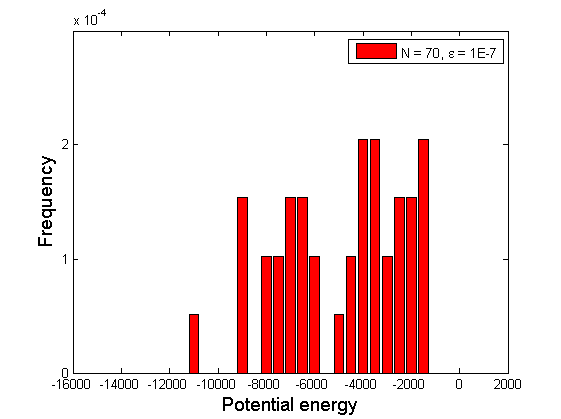
\includegraphics[width=1\linewidth]{Figures/epsilon7_pot.png}
\end{minipage}
\caption{
	Distribution of the kinetic and potential energy of bound particles in the star cluster after a time period of $1\tau_{crunch}$ with a step length of $1\times 10^{-4} \tau_{crunch}$ and $\epsilon = 1\times 10^{-2} \text{ ly}$ for 70 particles with normal distributed masses, uniformly distributed within a sphere generated by the functions presented in \secref{Method:GeneratingPosMassVel}. 
}
\label{fig:DistributionPotKinEnBoundHistograms2}
\end{figure}
	\section{The Dependence of Number of Particles on Radial Distribution}
\label{sec:NumberPartRadDist}
\tabref{tab:NumberPartRadDist} shows the dependence of number of particles on the average distance to the cluster center after reached equilibrium. 
From the table it seems that the final distance might be slightly increased when the number of particles increases. 
However, then is not a strong tendency. 
\begin{table}[H]
\centering
\begin{tabular}{|c|c|}
\hline
Number of particles  & Mean distance to center (ly)  \\
\hline
30 & 12.36
\\ \hline
50 & 13.69
\\ \hline
70 & 13.11
\\ \hline
100 & 14.75
\\ \hline
200 & 14.08
\\ \hline
\end{tabular}
\caption{
The average distance to the cluster center of bound particles after $3\tau_{crunch}$ with a step length of $10^{-4}\tau_{crunch}$ and $\epsilon = 10^{-7}$ for different numbers of particles bot same total mass.
}
\label{tab:NumberPartRadDist}
\end{table}
\begin{figure}[H]
\centering
\begin{minipage}{.5\textwidth}
  \centering
  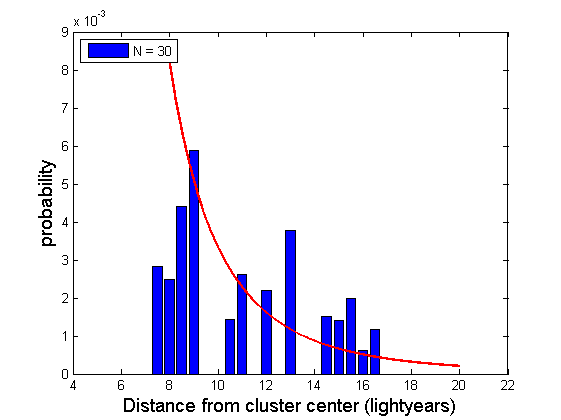
\includegraphics[width=1\linewidth]{Figures/N30.png}
\end{minipage}%
\begin{minipage}{.5\textwidth}
  \centering
  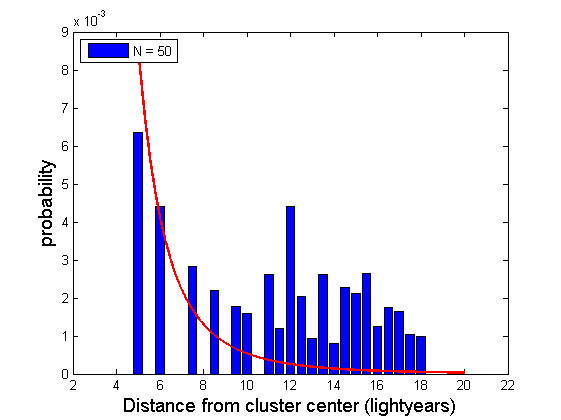
\includegraphics[width=1\linewidth]{Figures/N50.png}
\end{minipage}
\begin{minipage}{.5\textwidth}
  \centering
  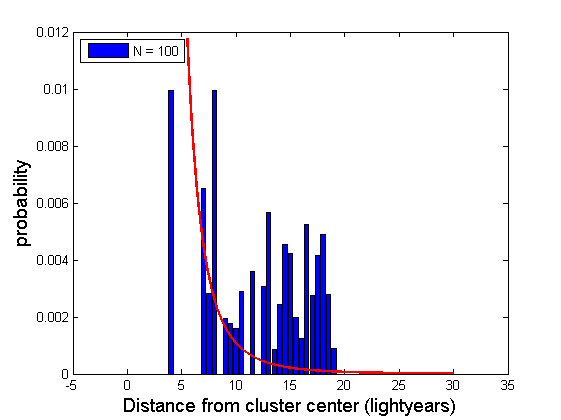
\includegraphics[width=1\linewidth]{Figures/N100.png}
\end{minipage}%
\begin{minipage}{.5\textwidth}
  \centering
  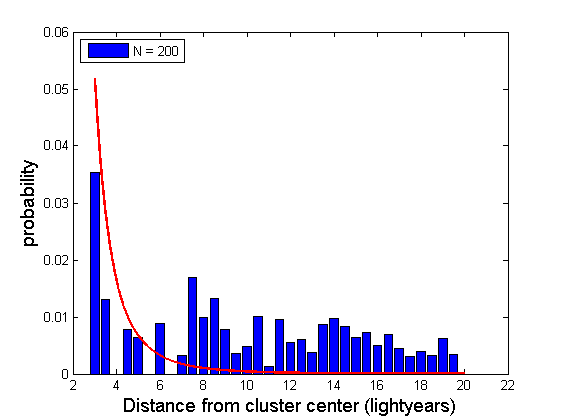
\includegraphics[width=1\linewidth]{Figures/N200.png}
\end{minipage}
\caption{
Radial density of bound particles after a time period of $3\tau_{crunch}$ plotted together with a fit computed from \matref{eq:radialDens}.
}
\label{fig:NumberPartRadDist}
\end{figure}
The histograms in \figref{fig:NumberPartRadDist} show the radial particle density for N = 30, 50, 100 and 200 (see \tabref{tab:NumberPartRadDist}).
The radial density is found by counting the number of particles at a distance $r_i$ from the center and dividing this by the sphere area, given as $4\pi r_i^2$ at this point, multiplied by the interval $dr$ that corresponds to the thickness of the bars in the histograms. 
The red curves are made to fit the radial density from the formula
\begin{align}
	n(r) = \frac{n_0}{\left( 1 0+ \left( \frac{r}{r_0} \right) ^4 \right)}
	\label{eq:radialDens}
	\end{align}
in which $n_0 \propto N^2$ and $r_0 \propto N^{-1/3}$
 \cite{ColdUniformSphericalCollapse}. 
The fit is not perfect, especially not for longer distances from the cluster center. 
However, the computed radial densities follow the appearance of the simple expression in \matref{eq:radialDens}.
	\chapter{Conclusion}




	% ¤¤ LITTERATURLISTE: SKAL VÆRE SIDST ¤¤
		\bibliographystyle{ieeetr}
		\bibliography{Bibtex/litteratur}

% ¤¤ BILAG: SKAL VÆRE ALLERSIDST ¤¤
	\appendix

	
\end{document}
